%fix pandoc 2.8 update


  \documentclass[oneside]{book}
%\documentclass[]{book}

\usepackage{lmodern}
\usepackage{setspace}
\setstretch{1.5}
\usepackage{amssymb,amsmath}
\usepackage{ifxetex,ifluatex}
\usepackage{fixltx2e} % provides \textsubscript
\ifnum 0\ifxetex 1\fi\ifluatex 1\fi=0 % if pdftex
  \usepackage[T1]{fontenc}
  \usepackage[utf8]{inputenc}
\else % if luatex or xelatex
  \ifxetex
    \usepackage{xltxtra,xunicode}
  \else
    \usepackage{fontspec}
  \fi
  \defaultfontfeatures{Ligatures=TeX,Scale=MatchLowercase}


\fi
% use upquote if available, for straight quotes in verbatim environments
\IfFileExists{upquote.sty}{\usepackage{upquote}}{}
% use microtype if available
\IfFileExists{microtype.sty}{%
\usepackage{microtype}
\UseMicrotypeSet[protrusion]{basicmath} % disable protrusion for tt fonts
}{}
\usepackage[a4paper, left=1.18in, right=1.18in, top=1.18in, bottom=0.787in]{geometry}
\usepackage[unicode=true]{hyperref}
\hypersetup{
            pdftitle={臺大論文模板},
            pdfauthor={廖永賦},
            pdfborder={0 0 0},
            breaklinks=true}
\urlstyle{same}  % don't use monospace font for urls
\usepackage{longtable,booktabs}
% Fix footnotes in tables (requires footnote package)
\IfFileExists{footnote.sty}{\usepackage{footnote}\makesavenoteenv{long table}}{}
\let\oldhref=\href
% Make links footnotes instead of hotlinks:
\renewcommand{\href}[2]{#2\footnote{\url{#1}}}
\IfFileExists{parskip.sty}{%
\usepackage{parskip}
}{% else
\setlength{\parindent}{0pt}
\setlength{\parskip}{6pt plus 2pt minus 1pt}
}
\setlength{\emergencystretch}{3em}  % prevent overfull lines
\providecommand{\tightlist}{%
  \setlength{\itemsep}{0pt}\setlength{\parskip}{0pt}}
\setcounter{secnumdepth}{5}

% set default figure placement to htbp
\makeatletter
\def\fps@figure{htbp}
\makeatother

\usepackage{pdfpages}
\usepackage{titlesec}
\usepackage{titletoc}
\usepackage{booktabs}
\usepackage{apptools}
\usepackage{float}
\usepackage[section]{placeins}

\usepackage[heading, fontset = none]{ctex}
\ctexset{appendix/name={\appendixname\space}}

\usepackage[fontsize=12pt]{scrextend}

% 如果想將每頁的頁碼置於中間下方,uncomment 下兩行
%\usepackage{fancyhdr}
%\pagestyle{fancy}

% Eng font-family
\setmainfont[
  Path=latex/,
  BoldFont={TimesNewRomanBold},
  ItalicFont={TimesNewRomanItalic},
  BoldItalicFont={TimesNewRomanBoldItalic}
]{TimesNewRoman}

% Trad Ch font-family
\setCJKmainfont[Path=latex/,AutoFakeBold=2.5,AutoFakeSlant=.3]{kaiti}
\setCJKmonofont[Path=latex/]{NotoSansMonoCJKtc}

% Special font: IPA
\newfontfamily{\ipa}[Path=latex/,AutoFakeBold=2.5,AutoFakeSlant=.3]{IPAfont} % Font for IPA symbols
\DeclareTextFontCommand{\ipatext}{\ipa}


%中文自動換行
\XeTeXlinebreaklocale "zh"
%文字的彈性間距
\XeTeXlinebreakskip = 0pt plus 1pt



\renewcommand{\figurename}{圖}
\renewcommand{\tablename}{表}
\renewcommand{\contentsname}{目錄}
\renewcommand{\listfigurename}{圖目錄}
\renewcommand{\listtablename}{表目錄}
\renewcommand{\appendixname}{附錄}
%\renewcommand{\bibname}{參考資料}

% deal with nuts floating figures
\renewcommand{\textfraction}{0.05}
\renewcommand{\topfraction}{0.8}
\renewcommand{\bottomfraction}{0.8}
\renewcommand{\floatpagefraction}{0.75}

\title{臺大論文模板}
\author{廖永賦}
\date{一月 13, 2021}


\usepackage{fontspec}
%使用xeCJK,其他的還有CJK或是xCJK
\usepackage{xeCJK}
\usepackage{bm}

% Set the default fonts
% See https://tug.org/pipermail/xetex/2011-March/020226.html for fontspec
% % \setmainfont[
%   Path=latex/,
%   BoldFont={TimesNewRomanBold.ttf},
%   ItalicFont={TimesNewRomanItalic.ttf},
%   BoldItalicFont={TimesNewRomanBoldItalic.ttf}
% ]{TimesNewRoman.ttf}
% 
% %     \setCJKmainfont[Path=latex/,AutoFakeBold=2.5,AutoFakeSlant=.3]{kaiti}
%     \setCJKmonofont[Path=latex/]{NotoSansMonoCJKtc}
% 


% IPA support (Works with linguisticsdown)
% 

\usepackage{xcolor}
\usepackage{transparent}







\begin{document}



\includepdf[pages={1}, scale=1]{front_matter/front_matter.pdf}

\clearpage
\pagenumbering{roman}

\phantomsection
\addcontentsline{toc}{chapter}{口試委員會審定書}

\includepdf[pages={1}, scale=1]{certification-scan.pdf}


\phantomsection
\chapter*{誌謝}
非常感謝網路上各個默默耕耘開發 open source 專案的大大們。
非常感謝網路上各個默默耕耘開發 open source 專案的大大們。
非常感謝網路上各個默默耕耘開發 open source 專案的大大們。

沒有這些既存的資源,這份模板是不可能出現的。沒有這些既存的資源,這份模板是不可能出現的。沒有這些既存的資源,這份模板是不可能出現的。沒有這些既存的資源,這份模板是不可能出現的。
\addcontentsline{toc}{chapter}{誌謝}


\phantomsection
\chapter*{摘要}
摘要\textbf{第 5 行}開始而且不能是空行。摘要\textbf{第 5 行}開始而且不能是空行。摘要\textbf{第 5 行}開始而且不能是空行。摘要\textbf{第 5 行}開始而且不能是空行。

新段落要在前面空一行。新段落要在前面空一行。新段落要在前面空一行。新段落要在前面空一行。新段落要在前面空一行。
\bigbreak

\noindent
\textbf{關鍵字:} 第二行開始、R Markdown、Bookdown、可重製研究
\addcontentsline{toc}{chapter}{中文摘要}

\phantomsection
\chapter*{Abstract}
The first line of the abstract starts on \textbf{line 5} and must not be blank. The first line of the abstract starts on \textbf{line 5} and must not be blank. The first line of the abstract starts on \textbf{line 5} and must not be blank.

A new paragraph of the abstract. A new paragraph of the abstract. A new paragraph of the abstract. A new paragraph of the abstract. A new paragraph of the abstract. A new paragraph of the abstract.
\bigbreak

\noindent
\textbf{Keywords:} Line 2, R Markdown, Bookdown, Reproducible Research
\addcontentsline{toc}{chapter}{英文摘要}


{
\setcounter{tocdepth}{1}
\tableofcontents
%\phantomsection
%\addcontentsline{toc}{chapter}{\contentsname}
}

\newpage

\listoftables
\phantomsection
\addcontentsline{toc}{chapter}{\listtablename}
\newpage

\listoffigures
\phantomsection
\addcontentsline{toc}{chapter}{\listfigurename}
\newpage

% Set independent linestretch for code chunks
\let\oldShaded=\Shaded
\let\endoldShaded=\endShaded
\renewenvironment{Shaded}{
      \begin{spacing}{1}\begin{oldShaded}
    }
  {
  \end{oldShaded}
  \end{spacing}
  }

\clearpage
\pagenumbering{arabic}

\hypertarget{ux7814ux7a76ux52d5ux6a5f}{%
\chapter{研究動機}\label{ux7814ux7a76ux52d5ux6a5f}}

失業率是一個衡量當下社會經濟狀況、人民生活水準的重要指標。不同國家都會公布各自的失業率,讓國民、企業或是政府了解當下的就業狀況。在台灣失業率是每月公布,相較於每季公布的國內生產毛額,經濟學家能藉由失業率的資料更即時的了解當下景氣的概況。

因此,能否藉由過往的失業狀況,推估預測未來幾個月內的失業率變化,對於政策制定與推行至關重要, Montgomery, Zarnowitz, Tsay, \& Tiao (\protect\hyperlink{ref-montgomeryForecastingUnemploymentRate1998}{1998}) 特別是在景氣的緊縮期,民眾會想了解緊縮持續的時間會持續多久與景氣的反轉點何時會出現。但 Montgomery et al. (\protect\hyperlink{ref-montgomeryForecastingUnemploymentRate1998}{1998}) 又因為失業率循環為非對稱性,線性模型相對於非線性模型,較無法精確地表現出非對稱的循環。

失業率指的是指15歲以上,有工作能力,且有工作意願但沒有工作機會的人口,佔本國人口扣除現役軍人、監管人口與失蹤人口後有工作能力,且有工作意願的比例。失業的原因可簡單分為四種,分別為摩擦性失業、結構性失業、季節性失業與自然失業,其中摩擦性失業指的是因為工作的傳換,暫時的失業;結構性失業,是指因產業的變動導致的失業;季節性失業,代表因為景氣的循環而造成的失業;自然失業則指,經濟體系內自然產生的失業。

從圖\ref{fig:unemm}台灣的失業率有些特別之處,失業率的時間序列上有某些大幅度的變化,回顧過去的歷史,可了解到這些結構性轉變的背後,隱含當下經濟社會甚至政治上所受到的影響。本研究探討的時間範圍為1978年1月至2019年12月間台灣失業率的變化。此階段經歷過1970年代的石油危機,1980年代的金融自由化,1990年代的亞洲金融風暴,2000年代加入世界貿易組織、金融海嘯,使得不同時期失業率皆有不同程度的變化,有些的影響短暫但也有造成長期失業率結構上的改變。

本研究藉由單變數的失業率資料,以差分整合移動平均自迴歸模型為基礎,建構兩種類神經網絡,比較三者在不同期數後,預測失業率上後的表現,期望可以找到優於差分整合移動平均自迴歸模型的非線性模型。

\hypertarget{ux6587ux737bux56deux9867}{%
\chapter{文獻回顧}\label{ux6587ux737bux56deux9867}}

預測是希望能預見未來,是為了可以未雨綢繆,提早安排。但預測並不是直接看到未來的水晶球,而是透過過去的狀況來推估未來的變化。預測可以分為兩種,分別是對當下經濟狀況的預測(nowcasting)與對未來經濟狀況的預測(forecast)。在 Montgomery et al. (\protect\hyperlink{ref-montgomeryForecastingUnemploymentRate1998}{1998}) 文章中指出,因為是藉由觀察資料來形成預測,因此預測可視為給定條件機率分配的估計問題。是一個把較複雜的資料生成步驟(data generating process)簡化,同時在可接受、可預期的損失和風險內,選擇能降低其損失值的參數模型。預測模型是藉由擷取資料的特徵並篩選掉資料中的噪音(Zhu \& Wu, \protect\hyperlink{ref-zhuClassNoiseVs2004}{2004}),來找出最合適的參數設定。 Elliott \& Timmermann (\protect\hyperlink{ref-elliottEconomicForecasting2008}{2008}) 也提到預測模型最好看成是一種近似或是追蹤的裝置,所以不應該期待預測模型會在不同時間下都表現良好。因此,預測其實是種估計,透過不同模型裡頭的參數,去描繪過去的狀況,推估未來的情形,但沒有一個模型是完美的,因為總有些參數是被隱藏著,等到事情發生時才會顯現,因此沒有永遠最好的模型。

總體經濟的預測,根據 Diebold (\protect\hyperlink{ref-dieboldPresentFutureMacroeconomic1998}{1998}) 可分為結構性與非結構性。結構性指的是藉由建立理論模型,並據此對實際資料進行預測,像是動態隨機一般均衡模型(Dynamic stochastic general equilibrium);而非結構性模型,則是對資料本身建立相對應的模型,進行後續資料的預測,像是向量自迴歸模型(Vector autoregression)。此外,非結構性模型較適合無條件的預測,不適合有條件的預測 Lucas (\protect\hyperlink{ref-lucasEconometricPolicyEvaluation1976}{1976}) 。本研究提及的方法,皆屬於非結構性模型。 Hall \& Cook (\protect\hyperlink{ref-hallMacroeconomicIndicatorForecasting2017}{2017}) 提及目前的總體指標預測多半是以線性模型為主,像是向量自迴歸模型(Vector autoregression)與差分整合移動平均自迴歸模型(Autoregressive Integrated Moving Average,ARIMA),差分整合移動平均自迴歸模型屬於非結構性模型,雖然對於模型資料生成假設較少,但差分整合移動平均自迴歸模型對於模型設定相對敏感,像是要加入多少個落後項。在本研究中會運用到的線性模型為季節差分整合移動平均自迴歸模型(Seasonal Autoregressive Integrated Moving Average, SARIMA),亦需要自行設定落後期數。

總體經濟狀況產生變化,當然也會反映在勞動市場上,我們從失業率的變化就可看出端倪。失業對個人或其家庭都是十分痛苦的一件事情,因此經濟學關於失業率的探討的面向十分廣泛, Layard, Nickell, \& Jackman (\protect\hyperlink{ref-layardUnemploymentMacroeconomicPerformance1991}{1991}) 提及像是失業的成因、政策上可以如何改善降低失業率、國與國之間失業率的比較和失業率等。關於失業率的預測有 Montgomery et al. (\protect\hyperlink{ref-montgomeryForecastingUnemploymentRate1998}{1998}) 提到失業率在景氣擴張期與收縮期時,不同時期不同預測方法的表現不同; Dritsaki (\protect\hyperlink{ref-dritsakiForecastSarimaModels2016}{2016}) 是用季節差分整合移動平均自迴歸模型來預測希臘的失業率,但沒有做結構性改變的設定。

此外, Coulombe, Leroux, Stevanovic, \& Surprenant (\protect\hyperlink{ref-coulombeHowMachineLearning2020}{2020}) 因為總體資料存在不確定性與金融摩擦, Elliott \& Timmermann (\protect\hyperlink{ref-elliottEconomicForecasting2008}{2008}) 提到建立模型時常發現時間序列資料是非定態的,類神經網絡的特點--非線性方式,特別是在做長期數的預測時,容易抓到這些特徵。 Coulombe et al. (\protect\hyperlink{ref-coulombeHowMachineLearning2020}{2020}) 儘管類神經網絡在總體經濟的運用已有一段歷史( Kuan \& White (\protect\hyperlink{ref-kuanArtificialNeuralNetworks1994}{1994}) , Swanson \& White (\protect\hyperlink{ref-swansonModelSelectionApproach1997}{1997}) , Stock \& Watson (\protect\hyperlink{ref-stockCointegrationCausalityForecasting1999}{1999}) ),但預測相關的文獻是最近隨著類神經網絡的演進而有大幅度的成長。 雖然 Coulombe et al. (\protect\hyperlink{ref-coulombeHowMachineLearning2020}{2020}) 提到在資料較少的模型中,非線性沒辦法顯著提升預測能力。

本研究會用到的類神經網絡有長短期記憶網絡及時序卷積網絡。 Hochreiter \& Schmidhuber (\protect\hyperlink{ref-hochreiterLongShortTermMemory1997}{1997}) 提出的\textbf{長短期記憶網絡},屬於循環神經網絡(Recurrent Neural Network, RNN)的一種,循環神經網絡具有記憶時間順序的功能,因此常被用來處理序列資料,如翻譯或語音處理等。此外, Bai, Kolter, \& Koltun (\protect\hyperlink{ref-baiEmpiricalEvaluationGeneric2018}{2018}) 彙整( Oord et al. (\protect\hyperlink{ref-oordWaveNetGenerativeModel2016}{2016}) , Dauphin, Fan, Auli, \& Grangier (\protect\hyperlink{ref-dauphinLanguageModelingGated2017}{2017}))並藉由以下特徵的第1點,精簡出另一個處理時間序列資料的類神經網絡架構--時序卷積網絡(Temporal Convolutional Networks, TCN),此架構下具備的特徵有

\begin{itemize}
\tightlist
\item
  1.卷積具有因果關係
\item
  2.可採用任意長度的序列資料,並能輸出出相同長度的序列,如同循環神經網絡一般。因而改善了卷積神經網絡對序列資料的處理。
\end{itemize}

在台灣失業率資料裡,可以看到不同時段間有長時間大幅度的變化,表示不同時段間可能有 Boot \& Pick (\protect\hyperlink{ref-bootDoesModelingStructural2020}{2020}) 提及的結構性變化。 Boot \& Pick (\protect\hyperlink{ref-bootDoesModelingStructural2020}{2020}) 有相當程度的結構性改變,在預測時將結構改變納入考量可以增進預測的能力,即便僅有2到3個結構改變點。因此在後續模型的處理上,都有考量結構性改變的處理,以改善模型預測上的能力。

\hypertarget{ux8cc7ux6599ux8207ux65b9ux6cd5}{%
\chapter{資料與方法}\label{ux8cc7ux6599ux8207ux65b9ux6cd5}}

本章節將介紹資料處理與方法,從傳統的統計量、統計檢定、時間序列模型SARIMA,再進到神經網路。

\hypertarget{ux8cc7ux6599}{%
\section{資料}\label{ux8cc7ux6599}}

台灣失業率,是由主計處的每月失業率原始資料,從1978年1月至2019年12月,選擇以十大建設開始後為時點至新冠病毒影響前,資料沒經過季節調整。資料分群的方式分做訓練、驗證及測試集,而SARIMA則將訓練與測試合併為訓練集。資料1978年1月至2008年3月作為訓練集,占總資料的70\%;資料2008年4月至2013年9月作為驗證集,共78筆,占總資料的15\%;資料2013年10月至2019年12月作為測試集,共75筆,占總資料的15\%。

神經網絡的資料分群是為了在偏差-方差權衡(Bias--variance tradeoff)中找到平衡點,也就是避免參數的估計只在訓練集有高度擬合,在測試集卻過度擬合,而透過驗證集協助訓練及訓練出的模型,在偏差與方差間調整,確保測試集中的預測狀況與訓練集不會相去太遠。

\[
Bias[\hat{f(x)}] = E[\hat{f(x)}-f(x)]
\]

\[
Variance[\hat{f(x)}] = E[(\hat{f(x)}-E[\hat{f(x)}])^2]
\]

\hypertarget{ux53f0ux7063ux5931ux696dux7387ux8da8ux52e2ux5716}{%
\section{台灣失業率趨勢圖}\label{ux53f0ux7063ux5931ux696dux7387ux8da8ux52e2ux5716}}

圖\ref{fig:unemm} 顯示1978年1月至2019年12月的台灣失業率,資料顯示此段期間資料型態可能有出現結構性的改變,在2003年1月資料中可見到較大的跳躍。

\begin{figure}

{\centering 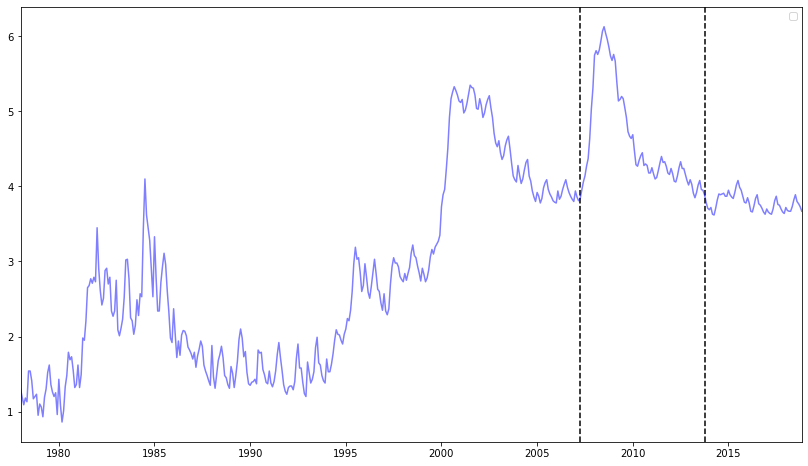
\includegraphics[width=.6\linewidth]{./fig/Unem} 

}

\caption{失業率趨勢圖}\label{fig:unemm}
\end{figure}

\hypertarget{ux985eux795eux7d93ux7db2ux7d61ux7684ux8cc7ux6599ux6a19ux6e96ux5316}{%
\section{類神經網絡的資料標準化}\label{ux985eux795eux7d93ux7db2ux7d61ux7684ux8cc7ux6599ux6a19ux6e96ux5316}}

將原始水準值轉換到{[}0,1{]}區間,可以加快類神經網絡的收斂速度。以下列方式進行標準化:
標準化方式為:原始水準值扣除最小值,再除以整體資料的分布範圍,也就是最大值減去最小值,以數學式表示如下:
(原始水準值 - 最小值)/(最大值 - 最小值),
但在最後判斷預測能力時,會轉換為相對於原始失業率的預測誤差。

\hypertarget{ux65b9ux6cd5}{%
\chapter{方法}\label{ux65b9ux6cd5}}

\hypertarget{ux55aeux6839ux8207ux5e73ux7a69ux6027ux6aa2ux5b9a}{%
\section{單根與平穩性檢定}\label{ux55aeux6839ux8207ux5e73ux7a69ux6027ux6aa2ux5b9a}}

因失業率為一時間序列,加上先前初步判斷有結構性的改變,本研究先檢定失業率是否具有單根(unit root)與結構性斷裂(structrual break)。
所謂結構性斷裂是指失業率在不同時段內有著不同的平均值,假設失業率的觀察值為\(y_t\),其中\(t=0,1,...T-1\),
\[y_t = u_t + z_t\]
\(u_t\)表示各段時間內失業率的平均值,\(z_t\)代表殘差項(誤差項?)\\
若在不同區間具有不同的失業率平均值,可表示如下,
\[
 u_t = 
  \begin{cases} 
   u_1, & 0 \leq t<t_1 \\
   u_2, & t_1 \leq t<t_2 \\
   \vdots \\
   u_{m+1}, & t_m \leq t<T-1
  \end{cases}
\]
其中\(t_1,t_2,...,t_m\)為平均值變動的時間點。

本研究藉由 Zivot \& Andrews (\protect\hyperlink{ref-zivotFurtherEvidenceGreat1992}{1992}) 的Zivot-Andrews檢定與 Bai \& Perron (\protect\hyperlink{ref-baiComputationAnalysisMultiple2003}{2003}) 的Bai-Perron檢定來做是否具有結構性斷裂的驗證。

Zivot-Andrews的目標是估計出,在趨勢和平穩(trend-stationary)的對立假設上權重最大的斷裂點。Zivot-Andrews檢定,修改Perron採用ADF單根檢定的策略,將PERRON假定外生的\(\lambda\)內生化,並透過\(t_{\hat{\alpha^i}}(\lambda)<\kappa_\alpha(\lambda)\)的t檢定來作為判斷的依據,其中\(\kappa_\alpha(\lambda)\)表示在固定的\(\lambda=T_B/T\)下的漸進分配。

Zivot-Andrews檢定的虛無假設為,

\[y_t = \mu+y_{t-1}+e_t\]

對立假設有三種,分別是具有一個均值的結構改變,

\[y_t=\hat{\mu^A}+\hat{\theta^A}DU_t(\hat{\lambda})+\hat{\beta^A}t+\hat{\alpha^A}y_{t-1}+\sum\limits^k_{j=1}\hat{c_j^A}\delta y_{t-j}+\hat{e_t}\]

具有斜率趨勢改變,

\[y_t=\hat{\mu^B}+\hat{\beta^B}t+\hat{\gamma^B}DT^*_t(\hat{\lambda})+\hat{\beta^B}t+\hat{\alpha^B}y_{t-1}+\sum\limits^k_{j=1}\hat{c_j^B}\delta y_{t-j}+\hat{e_t}\]

具有結構與趨勢改變,

\[y_t=\hat{\mu^C}+\hat{\theta^C}DU_t(\hat{\lambda})+\hat{\beta^C}t+\hat{\gamma^C}DT^*_t(\hat{\lambda})+\hat{\alpha^C}y_{t-1}+\sum\limits^k_{j=1}\hat{c_j^C}\delta y_{t-j}+\hat{e_t}\]

其中,\(DU_t=1\)如果\(t>T\lambda\),其他狀況\(DU_t=0\)表示在可能的結構斷裂時間(\(T_B=T\lambda\))上,均值的移動。\(DT^*_t(\hat{\lambda})=t-T\lambda\)如果\(t>T\lambda\),其他況狀則\(DT^*_t(\hat{\lambda})=0\),表示斜率的變動。

在Zivot-Andrews檢定的統計量為-5.898,小於臨界值\(\alpha\)=0.01時的-5.57,因此拒絕H0虛無假設,失業率資料為定態但有結構性斷裂。

而 Bai \& Perron (\protect\hyperlink{ref-baiComputationAnalysisMultiple2003}{2003}) 提出的Bai-Perron檢定,則是用來檢測是否具有多個結構性斷裂點,相較於Zivot-Andrews檢定,Bai-Perron檢定還可以標定多個結構性斷裂點發生的時間為何。

假設以下的迴歸式有m個斷裂點(m+1個區間)

\[y_t=z_t^{'}\delta_j+u_t,t=T_{j-1}+1,...T_j\]
對\(j=1,...,m+1\)此處的\(y_t\)表示在t期的被解釋變數、\(z_t\)(q*1)為共變量(covariates)、結構改變點\((T_1,..,T_m)\)視為未知。目標是要同時估計參數與未知的結構改變點。藉由最小平方法則(least-square principle)對每一個m-分割區間,由以下的式子透過極小化殘差的平方和,估計出相對應的\(\delta_j\),

\[S_T(T_1,...T_m)=\sum\limits_{i=1}^{m+1}\sum\limits_{t=T_i+1}^{T_t}[y_t-z_t^{'}\delta_i]^2\]

先估計出最小的\((\hat{T_1},...\hat{T_m})\),

\[(\hat{T_1},...\hat{T_m}) =\mathop{\arg\min_{T_1,...T_m}} S_T(T_1,...T_m)\]

再將估計出的\((\hat{T_1},...\hat{T_m})\)代回前式中,估計出\(\hat{\delta}=\hat{\delta}(\hat{T_1},...\hat{T_m})\)與\(\hat{\beta}=\hat{\beta}(\hat{T_1},...\hat{T_m})\),最終則是在給定的斷裂點數\(m\)下,藉由動態規劃 (Dynamic programming)的方法找出殘差均方和(Residual sum of sqaure)最小的線性組合,則為該斷裂數下最佳解。接著再以supF type test 來檢定0,l個斷裂點與l,l+1個斷裂點直到m個斷裂點下,檢視模型選擇準則BIC直最小的斷裂點數,即為Bai-Perron檢定最適的結構斷裂點數。

模型選擇標準BIC,選取BIC值最小者為最適合的模型,

\[BIC = k\ln(n)-2\ln(\hat L)\]

其中k為模型參數個數、n為樣本數大小、\(\hat L\)為最大概似函數值。\\
藉由R的urca套件內的breakpoints函數(Zeileis, Kleiber, Krämer, \& Hornik, \protect\hyperlink{ref-zeileisTestingDatingStructural2003}{2003}),由表\ref{tab:BP} 找出最小的選BIC在4個結構性斷裂處,因此失業率資料考量4個結構性斷裂點。因此,本研究以加入虛擬變數(dummy variable)來做資料上的處理。

\begin{table}

\caption{\label{tab:BP}Bai-Perron檢定}
\centering
\begin{tabular}[t]{l|l|r}
\hline
結構變化的個數 & 結構變化時點 & BIC\\
\hline
1 & 2000(9) & 1013\\
\hline
2 & 1994(11) 2001(2) & 948\\
\hline
3 & 1995(1) 2001(4) 2011(11) & 872\\
\hline
4* & 1987(12) 1995(1) 2001(4) 2011(11) & 846\\
\hline
5 & 1987(12) 1994(12) 2001(3) 2007(6) 2013(9) & 861\\
\hline
\end{tabular}
\end{table}

從表\ref{tab:BP}可得知,1978年1月至2019年12月存在4個結構性斷裂點,分別為1987年12月、1995年1月、2001年4月 與2011年11月,從圖\ref{fig:unemm}回顧這段時間的歷史,在這些結構性斷裂點的前後,藉由國家發展委員會的歷次景氣循環認定工作\footnote{\url{https://www.ndc.gov.tw/Content_List.aspx?n=D343A0AE4FE52D43}},可以略知這段期間所發生的一些事件。在1979年,第二次石油危機,1980年代後期,台灣經濟高速發展,國際熱錢流入,外匯儲備上升到1987年的768億美元,促使金融自由化,像是財政部並於1990年4月發布「商業銀行設立標準」,接受新銀行設立申請,此時正是台灣錢淹腳目的時代,失業率降至此區間的低點。1997年7月開始的亞洲金融風暴。2001年3月開始的網路泡沫破滅,再加上2001年9月的911事件,使得失業率有大幅度的躍升。2008年下半年,美國次級房貸引發金融海嘯,導致失業率急遽升高。2010年年初,則發生歐洲主權債務危機。

\hypertarget{ux4ee5ux8ff4ux6b78ux79fbux9664ux7d50ux69cbux6027ux65b7ux88c2ux9edeux7684ux6548ux679c}{%
\section{以迴歸移除結構性斷裂點的效果}\label{ux4ee5ux8ff4ux6b78ux79fbux9664ux7d50ux69cbux6027ux65b7ux88c2ux9edeux7684ux6548ux679c}}

\hypertarget{ux985eux795eux7d93ux7db2ux7d61ux7684ux65b9ux6cd5}{%
\subsection{類神經網絡的方法}\label{ux985eux795eux7d93ux7db2ux7d61ux7684ux65b9ux6cd5}}

將失業率\(y_t\)對截距項與4個虛擬變數同時跑迴歸,

\begin{equation} 
  y_t = \beta_0+ \beta_1D_{1t}+\beta_2D_{2t}+\beta_3D_{3t}+\beta_4D_{4t}+z_t
  \label{eq:zt}
\end{equation}
其中,\(T\)為2019年12月的時點,\(D_1 = [D_{11},..D_{1t}...D_{1T}]^{'}\)在1988年9月至1995年1月間為1其餘為0的向量、\(D_2\)為在1995年2月至2001年4月間為1其餘為0的向量、\(D_3\)為在2001年5月至2011年11月間為1其餘為0的向量、\(D_4\)為2011年12月至2019年112月間為1其餘為0的向量、\(z_t\)為殘差項(residuals)。接著取出殘差項\(z_t\),以此做為下來預測誤差的真實值,與之後估計出 \(\hat{\epsilon}\) 的差值 \(|z_t-\hat{\epsilon}|\) 作為預測的誤差。

\hypertarget{ux5177ux7d50ux69cbux65b7ux88c2ux7684ux5b63ux7bc0ux6027ux5deeux5206ux6574ux5408ux79fbux52d5ux5e73ux5747ux81eaux8ff4ux6b78ux6a21ux578b}{%
\subsection{具結構斷裂的季節性差分整合移動平均自迴歸模型}\label{ux5177ux7d50ux69cbux65b7ux88c2ux7684ux5b63ux7bc0ux6027ux5deeux5206ux6574ux5408ux79fbux52d5ux5e73ux5747ux81eaux8ff4ux6b78ux6a21ux578b}}

具結構斷裂的季節性差分整合移動平均自迴歸模型(SARIMAX)模型為季節性差分整合移動平均自迴歸模型(seasonal autoregressive integrated moving average, SARIMA)同時加上虛擬變數的模型,
將失業率\(y_t\)對截距項與4個虛擬變數與SARIMA\textbf{同時}跑迴歸,
根據 US Census Bureau (\protect\hyperlink{ref-uscensusbureauX13ARIMASEATSSeasonalAdjustment2017}{2017}) 寫成時變均值(time-varying mean)函數,

\[\Phi_P(B^s)\phi_p(B)(1-B)^d(1-B^s)^D (y_t-\sum_i \beta_ix_{it}) = \theta_q(B)\Theta_Q(B^s)\varepsilon_t\]

符號表示同上述類神經網絡的方法。

而SARIMA模型,Box-Jenkins SARIMA模型,以落後項(lag)表示模型為

\[\Phi_P(B^s)\phi_p(B)(1-B)^d(1-B^s)^D z_t = \theta_q(B)\Theta_Q(B^s)\varepsilon_t\]

其中,B是落後運算元,即\(Bz_t=z_{t-1}\);s代表季節周期整數;\(\phi_p(.),\theta(.),\Phi_p(.),\Theta(.)\)為落後運算子多項式,
對p,q\\
\[\phi_p(B) = 1-\phi_1B-\phi_2B^{2}-...-\phi_{p}B^{p}\]

\[\theta_q(L) = 1-\theta_1B-\theta_2B^{2}-...-\theta_qB^{q}\]
,對季節性P,Q
\[\Phi_P(B^s) = 1-\Phi_1B^s-\Phi_2B^s-...-\Phi_{P}B^{Ps}\]

\[\Theta_Q(L) = 1-\Theta_1B^s-\Theta_2B^{2s}-...-\Theta_QB^{Qs}\]

參考 Wei (\protect\hyperlink{ref-weiTimeSeriesAnalysis2005}{2005}) 表示方式,表示為\(ARIMA(p,d,q)(P,D,Q)_s\)。

\hypertarget{ux6311ux9078ux6700ux4f73ux7684ux5177ux7d50ux69cbux65b7ux88c2ux7684ux5b63ux7bc0ux6027ux5deeux5206ux6574ux5408ux79fbux52d5ux5e73ux5747ux81eaux8ff4ux6b78ux6a21ux578b}{%
\section{挑選最佳的具結構斷裂的季節性差分整合移動平均自迴歸模型}\label{ux6311ux9078ux6700ux4f73ux7684ux5177ux7d50ux69cbux65b7ux88c2ux7684ux5b63ux7bc0ux6027ux5deeux5206ux6574ux5408ux79fbux52d5ux5e73ux5747ux81eaux8ff4ux6b78ux6a21ux578b}}

上述提及具結構斷裂的季節性差分整合移動平均自迴歸模型的原理,本研究使用 Hyndman \& Khandakar (\protect\hyperlink{ref-hyndmanAutomaticTimeSeries2008}{2008}) 開發的 R套件\texttt{auto.arima}進行模型選擇,其中運用到Hyndman-Khandakar演算法,藉由選模準則AICc(Akaike Information Criterion correction) 挑選出AICc的最小值,以此為迴歸殘差配似最佳的具結構斷裂的季節性差分整合移動平均自迴歸模型模型。AICc是在小樣本下對AIC的修正。
\[AIC = -2logL+2m\]

其中m=p+q+P+Q,模型內的參數和,L是最大概似函數。

\[AICc = AIC+\frac{2k(k+1)}{n-k-1}\]

其中n為樣本數大小,k為參數個數,當n越大時,AICc會趨近於AIC。選出的模型為\(ARIMA(2,0,1)(2,0,0)_{12}\),各參數為

\begin{table}

\caption{\label{tab:SARIMAX}SARIMAX的參數}
\centering
\begin{tabular}[t]{l|r|r|l}
\hline
參數 & 估計值 & 標準誤 & AIC\\
\hline
intercept & 0.81 & 0.50 & -330.45\\
\hline
ar1 & 1.89 & 0.05 & BIC\\
\hline
ar2 & -0.90 & 0.04 & -285.78\\
\hline
ma1 & -0.85 & 0.06 & \\
\hline
sar1 & 0.37 & 0.05 & \\
\hline
sar2 & 0.32 & 0.05 & \\
\hline
虛擬變數1 & 0.66 & 0.14 & \\
\hline
虛擬變數2 & -0.46 & 0.20 & \\
\hline
虛擬變數3 & -2.29 & 0.25 & \\
\hline
虛擬變數4 & -1.48 & 0.29 & \\
\hline
\end{tabular}
\end{table}

\hypertarget{ux6aa2ux5b9aux6b98ux5deeux662fux5426ux6709ux975eux7ddaux6027}{%
\section{檢定殘差是否有非線性}\label{ux6aa2ux5b9aux6b98ux5deeux662fux5426ux6709ux975eux7ddaux6027}}

因本研究運用類神經網絡預測失業率,而類神經屬於非線性模型,本研究先檢定失業率的迴歸,式子\eqref{eq:zt}的殘差\(z_t\)是否為非線性,以了解非線性模型是否適用於預測失業率的模型中。本研究透過 Lee, White, \& Granger (\protect\hyperlink{ref-leeTestingNeglectedNonlinearity1993}{1993}) 提出的 White神經網絡檢定(White Neural Network Test)與 Teräsvirta, Lin, \& Granger (\protect\hyperlink{ref-terasvirtaPowerNeuralNetwork1993}{1993}) 提出的Teraesvirta神經網絡檢定(Teraesvirta Neural Network Test),來了解失業率的迴歸殘差非線性,在當期失業率的迴歸殘差與不同落後期數失業率的迴歸殘差之間的線性與非線性狀況。

Lee et al. (\protect\hyperlink{ref-leeTestingNeglectedNonlinearity1993}{1993}) 的White神經網絡檢定
假設在輸入(\(\tilde{x^{'}_t}\theta\))與輸出值(\(o\))之間,含有一層隱藏層。可表示為

\[o=\tilde{x^{'}_t}\theta+\sum\limits^q_{j=1}\beta_j\psi(\tilde{x^{'}_t}\gamma_j)\]

其檢定的虛無假設為
資料平均為線性(linearity in ``mean'')

\[H_0=P[E(y_t|X_t)=\tilde{X^{'}_t}\theta^{*}]=1\]
對某些\(\theta^{*}\)。
再將其套入Lagrange multiplier test後可表示為

\[H_0^{'}=E(\Psi_t\hat{e}_t)=0\]

,對立假設則為資料平均為非線性。

\[H_1^{'}=E(\Psi_t\hat{e}_t)\neq0\]

其中\(\hat{e}_t=y_t-\tilde{X^{'}_t}\hat{\theta}\)。衍伸的統計量可表示為,

\[M_n=(n^{-1/2}\sum\limits^n_{t=1}\Psi_t\hat{e}_t)^{'}\hat{W}^{-1}_n(n^{-1/2}\sum\limits^n_{t=1}\Psi_t\hat{e}_t)\]
其中、\(\Psi_t=(\psi (\tilde{X^{'}_t}\Gamma_1)),...,\psi (\tilde{X^{'}_t}\Gamma_q))^{'}\)、\(\hat{W}^{-1}_n\)為\(W^{*}=var(n^{-1/2}\sum\limits^n_{t=1}\Psi_t\hat{e}_t)\)的一致性估計值。因此可得,在虛無假設下\(M_n \to \chi^2(q)\)分配收斂,當\(n \to \infty\)。

在\(\alpha=0.05\)下,在落後期數為一期時,p-value為0.0468,拒絕線性假設;而在落後期數為兩期時,p-value0.0168,拒絕失業率為線性模型。

terasvirtaPowerNeuralNetwork1993 的Teraesvirta神經網絡檢定(Teraesvirta Neural Network Test)

在\(\alpha=0.05\)下,在落後期數為一期時,p-value為0.0513,,雖沒有拒絕線性假設,但已落在拒絕域的邊緣;而在落後期數為兩期時,p-value為0.01093,拒絕失業率為線性模型。
由White神經網絡檢定與 Teraesvirta神經網絡檢定,可知失業率資料存有非線性關係,因此,本研究後續嘗試以類神經網絡進行預測,查看是否有更好的預測效果、更少的預測誤差。

\hypertarget{ux7c21ux4ecbux985eux795eux7d93ux7db2ux7d61}{%
\section{簡介類神經網絡}\label{ux7c21ux4ecbux985eux795eux7d93ux7db2ux7d61}}

類神經網絡使預測上以非線性的模型進行預測,經過非線性檢定後具有非線性的迴歸殘差,在神經網絡可能會有較線性模型,也就是先前提及的SARIMAX模型,有更好的預測效果。

類神經網絡的精神是模仿神經元接受並藉由非線性的活化函數(activation function)來決定訊號的傳遞,激勵函數將線性關係轉為非線性,因為有非線性的轉換,就可以經由隱藏層來表示輸入值與輸出值間的關係,否則若仍為線性的活化函數仍能以無隱藏層的方式表示,如\(h(x)=cx\),則\(y(x)=h(h(x))=c^2x\)。透過多個節點以及層級的堆疊,達到學習輸入值(input)與輸出值(output)間的抽象關係。類神經網絡可分為三層,依序分別是輸入層、隱藏層及輸出層。

其中,類神經網絡的參數藉由反向傳播進行權重的更新,透過計算權重變化如何使輸出值(\(\hat{z_t}\))與真實值(\(z_t\))間的誤差變化縮小。反向誤差讓即便是複雜的神經網絡,也不必直接寫出誤差函數,也可以計算出不同權重變化下的誤差(或稱梯度)變動。

本研究以兩種類神經網絡與SARIMAX模型作為比較對象,分別是長短期記憶網絡(Long Short Term Memory, LSTM)與時序卷積網絡(Temporal Convolutional Networks, TCN)。本研究假設\(\hat{z_t}\)可表示為落後項變數的非線性函數,將神經網絡表示如下數學式,

\begin{equation} 
  \hat{z_t} = f(z_{t-1},...,z_{t-p})
  \label{eq:nn}
\end{equation}
,其中\(f(.)\)為本研究選擇的類神經網絡。

\hypertarget{ux9577ux77edux671fux8a18ux61b6ux7db2ux7d61}{%
\section{長短期記憶網絡}\label{ux9577ux77edux671fux8a18ux61b6ux7db2ux7d61}}

長短期記憶網絡由 Hochreiter \& Schmidhuber (\protect\hyperlink{ref-hochreiterLongShortTermMemory1997}{1997}) 提出,屬於循環神經網絡(Recurrent Neural Network, RNN)的一種,具有記憶時間順序的功能,因此常被用來處理序列資料,如翻譯或語音處理等,本研究的標的失業率也具有時間先後的數列,適合使用長短期記憶網絡來做預測。若將長短期記憶網絡應用在\eqref{eq:nn}上 ,令\(x_t=[z_{t-1},...,z_{t-p}]^T\)為第t期的輸入值(input),則可依長短期記憶網絡文獻(如 Merity, Keskar, \& Socher (\protect\hyperlink{ref-merityRegularizingOptimizingLSTM2017}{2017}) )表示成如下數學式,

\begin{equation} 
  i_t = \sigma_g(W^ix_t+U^ih_{t-1}) 
  \label{eq:InputGate}
\end{equation}

\begin{equation} 
  f_t = \sigma_g(W^fx_t+U^fh_{t-1})
  \label{eq:ForgetGate}
\end{equation}

\begin{equation} 
  o_t = \sigma_g(W^ox_t+U^oh_{t-1})
  \label{eq:OutputGate}
\end{equation}

\begin{equation} 
   \tilde{c_t} =\tanh(W^cx_t+U^ch_{t-1})
  \label{eq:tildeC}
\end{equation}

\begin{equation} 
   c_t = i_t \odot \tilde{c_t}+ f_t \odot c_{t-1}
  \label{eq:ct}
\end{equation}

\begin{equation} 
   h_t = o_t \odot \tanh(c_t)
  \label{eq:ht}
\end{equation}

\begin{equation} 
   \hat{z_t} = W^zh_t
  \label{eq:hatZ}
\end{equation}

其中\(h_t\)為當期的隱藏狀態(hidden state);\(c_t\)為記憶單元狀態(memory cell state);\(\hat{z_t}\)為對\(z_t\)的預測值。在式子\eqref{eq:InputGate}

\eqref{eq:OutputGate}中,\(i_t,f_t,o_t\)別代表輸入閥(Input Gate)、遺忘閥(Forget Gate)與輸出閥(Output Gate)。在式子中,\([W^i,W^f,W^o,U^i,U^f,U^o]\)為權重矩陣,而\(\sigma(.)\)
為Sigmoid函數,即

\[
\sigma(x)=\frac{1}{1+\exp(-x)}
\]

,\(i_t,f_t,o_t\)的值經Sigmoid函數作用後,會落在\((0,1)\)之間。候選值\(\tilde{c_t}\)是由式子\eqref{eq:tildeC} 來更新,而\(\tilde{c_t}\)是先將\(x_t, h_{t-1}\)以權重矩陣\(W^c,U^c\)進行線性組合後,再放入雙曲正切函數(\(\tanh\))轉換出候選值\(\tilde{c_t}\),其中雙曲正切函為,

\[\tanh(x) = \frac{\exp(x)-\exp(-x)}{\exp(x)+\exp(-x)}\]

經此轉換後,\(\tilde{c_t}\)會落在\((-1,1)\)的區間內。式子\eqref{eq:ct} 是將\(\tilde{c_t}\)通過輸入閥\(i_t\)後的值,與前一期的記憶單元狀態\(c_{t-1}\)經過遺忘閥留下的值,兩者加總後會被保留在當期的記憶單元狀態中。此處的\(\odot\)代表兩個向量間逐個元素(element-by-element)相乘。式子\eqref{eq:OutputGate} 顯示當期的記憶單元狀在\(\tanh\)轉換後,再經過輸出閥\(o_t\)後的當期的隱藏狀態。最後,從式子\eqref{eq:hatZ} 中,我們可以得到經過由當期的隱藏狀態,經過權重矩陣\(W^z\)進行線性組合後,得到的\(z_t\)的預測值\(\hat{z_t}\)。

\hypertarget{ux9577ux77edux671fux8a18ux61b6ux7db2ux7d61ux7684ux53c3ux6578ux8a2dux5b9a}{%
\subsection{長短期記憶網絡的參數設定}\label{ux9577ux77edux671fux8a18ux61b6ux7db2ux7d61ux7684ux53c3ux6578ux8a2dux5b9a}}

長短期記憶網絡的輸入值為當期失業率與前\(T\)期的落後項,預測的比對值也就是預測的真實值為h期後的失業率。以函數表示如下,

\[
\hat{y_{t+h}} = f(y_t, y_{t-1}, ..., y_{t-T})
\]

因此長短期記憶網絡的目標是降低預測的比對值\(\hat{y_{t+h}}\)與真實值為h期後的失業率\(y_{t+h}\)兩者間的誤差。此長短期記憶網絡共使用了266個參數來做估計。

長短期記憶網絡的優點有,可將記憶分為長短期儲存,是種經過改良後的循環神經網絡模型,優於簡單的循環神經網絡模型,不會因為梯度的爆炸或是消失,導致訓練上的問題。但長短期記憶網絡的缺點是,模型訓練時間較長、較易過度擬合(overfitting),因此本研究使用 Merity et al. (\protect\hyperlink{ref-merityRegularizingOptimizingLSTM2017}{2017}) 的非同步隨機梯度下降的權重捨棄的長短期記憶網絡(Asynchronous Stochastic Gradient Descent Weight-Dropped LSTM, AWD-LSTM)來處理過度擬合的問題。本研究採用單層的非同步隨機梯度下降的權重捨棄的長短期記憶網絡,因為在訓練的結果上單雙層預測的差異不大,避免層數多、參數多而造成過度擬合的狀況,同時節省訓練的時間。

在非同步隨機梯度下降的權重捨棄的長短期記憶網絡(AWD-LSTM))中,共有4個調整過度擬合的參數設定,分別是權重捨棄(Weight Dropouted)、變分丟棄法(Variational Dropout)、激活正規化(activation regularisation)、暫時激活正規化(temporal activation regularisation),後兩者屬於\(L_2\)範數(norm)。因為循環網絡上運用丟棄法(drop out) 需特別注意,不能隨機丟棄每個時點的隱藏狀態,因為會損害循環網絡在時間順序上。

見圖\ref{fig:LSTMmodel}所示,權重捨棄使用的是捨棄連結(DropConnect)的方式,捨棄連結將輸入進模型中,隨機選擇子集的權重調整為;變分丟棄法,是根據貝氏學習理論(Bayesian learning)的方式,對參數\(\theta\)的抽樣,而每次抽樣到的參數在同一個訓練回合中都保持固定,以固定遮罩的方式維持每次訓練中參數的一致,應用上是將丟棄隱藏層(dropout hidden)分別用在長短期記憶網絡層與層之間和最後的輸出值\(z_t\)上,因本研究僅使用單層的長短期記憶網絡,因此僅至於輸出層前;激活正規化是對顯著大於0的激活進行懲罰、暫時激活正規化則是避免最後兩層的隱藏層差太多,兩者都僅使用在最後一個長短期記憶網絡上與輸出層上,因本研究為單層的長短期記憶網絡,所以只設置於隱藏層\(h_t\)與輸出層\(z_t\)之間。

\begin{figure}

{\centering 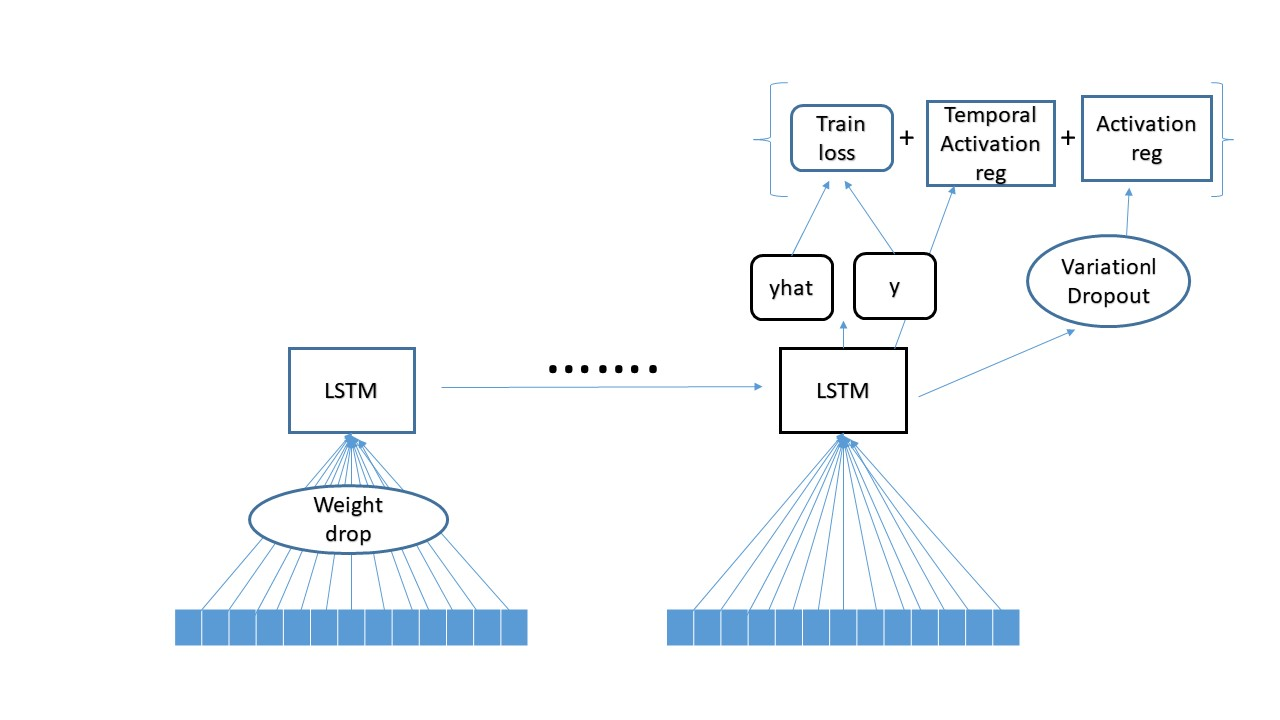
\includegraphics[width=.6\linewidth]{./fig/LSTM_model} 

}

\caption{AWDLSTM示意圖}\label{fig:LSTMmodel}
\end{figure}

爾後,在落後12,13,14,15,16期、LSTM為1,2層、隱藏層節點為4,6,8、權重捨棄在0.1,0.3、變分丟棄法為0.2,0.4、激活正規化在1.0,1.5,2.0、暫時激活正規化在1.0,1.5,2.0下,挑選出驗證集中均方根誤差最小者為最適參數,每種參數組合跑10次,每次訓練1000回,再從10次間挑選出其中位數代表該種組合的表現。最後挑選出的是落後12期、LSTM為1層、隱藏層節點為4、權重捨棄0.3、激活正規化1.5、暫時激活正規化1.50,作為預測用的非同步隨機梯度下降的權重捨棄的長短期記憶網絡(AWD-LSTM)),共使用266個參數。

\hypertarget{ux6642ux5e8fux5377ux7a4dux7db2ux7d61}{%
\section{時序卷積網絡}\label{ux6642ux5e8fux5377ux7a4dux7db2ux7d61}}

以 Bai et al. (\protect\hyperlink{ref-baiEmpiricalEvaluationGeneric2018}{2018}) 彙整出的時序卷積網絡(Temporal Convolutional Networks, TCN),讓卷積神經網絡(Convolutional Neural Network, CNN)也能在時間序列的處理上有好的表現。卷積神經網絡是將各個資料經過卷積,卷積可視為加權後,作為神經網絡的輸入值,並經多次堆疊而成的神經網絡。因此,代表卷積神經網絡不是以單點為輸入,而是以一群被卷積的資料為輸入值,這可以加大網絡對於資料區塊上的認識。

時序卷積網絡改善了卷積神經網絡對序列資料的處理,時序卷積網絡主要是建立在兩個概念上,分別是一維的全連接層(Fully Convolution Network)與因果卷積層(Causal Network)。一維的全連接層使時序卷積網絡將自動補零(padding),使得經過卷積後仍會維持相同的長度。若不補零,則會退化為 Waibel, Hanazawa, Hinton, Shikano, \& Lang (\protect\hyperlink{ref-waibelPhonemeRecognitionUsing1989}{1989}) 提出的模型,此退化模型不利於多個卷積層堆疊,容易過度擬和。而改進後有補零的模型,因為卷積核不會受到被卷積個數長度的影響,更適合做多層卷積的疊加。再者,因果卷積層的設置,確保未來的資訊不會逆流到過去,確保每個時點卷積的輸出值,不會使用到未來的資訊,如\ref{fig:causal}摘自 Bai et al. (\protect\hyperlink{ref-baiEmpiricalEvaluationGeneric2018}{2018}) 的文章。

\begin{figure}

{\centering \subfloat[沒有因果關係\label{fig:causal-1}]{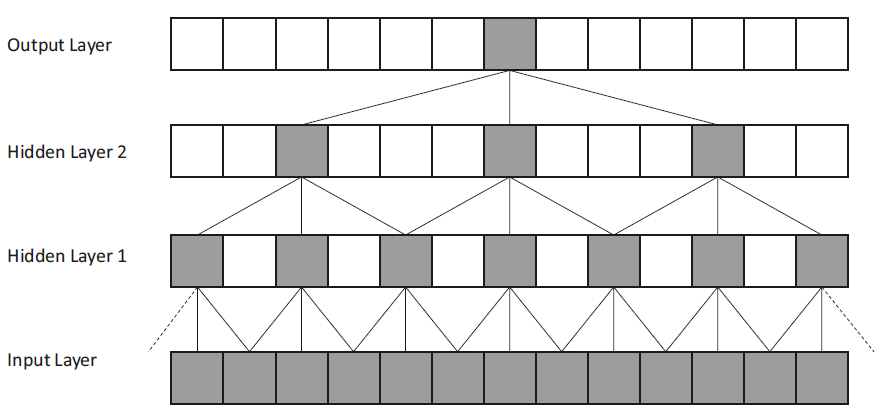
\includegraphics[width=.5\linewidth]{./fig/acausal} }\subfloat[有因果關係\label{fig:causal-2}]{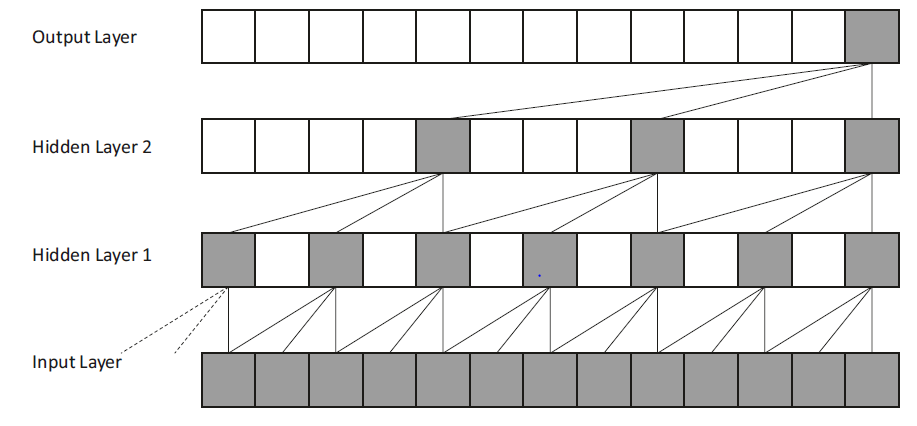
\includegraphics[width=.5\linewidth]{./fig/causal} }

}

\caption{因果關係}\label{fig:causal}
\end{figure}

以數學式表示,假設\(x=\{x_0,x_1,...x_{T-1}\}\)為一T期的時間序列,\(\omega = \{\omega_0,\omega_1,..,\omega_{k-1}\}\)為大小等於k的一維卷積核(kernel),且\(k<T\)。使用卷積核\(\omega\)對\(x\)序列做卷積,可得數列\(\{\Omega(t)\}_{t=0}^{T-1}\),定義為
\begin{equation} 
   \Omega(t) = \omega_0x_t+\omega_1x_{t-1}+\omega_1x_{t-2}+...+\omega_{k-1}x_{t-(k-1)}
  \label{eq:tcn}
\end{equation}

,在\(t=0\)時,\(x_0\)之前的變數均設為0,即
\begin{equation} 
   x_{-1}=x_{-2}=...=x_{-(k-1)}=0
  \label{eq:padding}
\end{equation}

此外,為了擴大卷積層有效的感受域(respective field),時序卷積網絡會使用的是膨脹卷積(dilated convolution),放大被卷積元素之間的距離,形成 Oord et al. (\protect\hyperlink{ref-oordWaveNetGenerativeModel2016}{2016}) 提出的具因果關係的膨脹卷積。此時,式子\eqref{eq:tcn}要修改為,

\begin{equation} 
   \Omega_d(t) = \omega_0x_t+\omega_1x_{t-d}+\omega_1x_{t-2d}+...+\omega_{k-1}x_{t-(k-1)d}
  \label{eq:tcnd}
\end{equation}

其中,整數d為膨脹因子(dilation factor),而相對的式子\eqref{eq:tcn}也要改為,
\begin{equation} 
   x_{-d}=x_{-2d}=...=x_{-(k-1)d}=0
  \label{eq:paddingd}
\end{equation}

式子\eqref{eq:tcnd}是蒐集時點\(t,t-d,...t-(k-1)d\)的輸入值做加權,輸入值兩兩相隔d期,膨脹卷積又稱為空洞(atrous)卷積。當\(d=1\)時,便回到與式子\eqref{eq:tcn}相同的一般卷積,又稱做稠密(dense)卷積。

研究者通常會設計多層的時序卷積網絡,藉由膨脹因子讓越高層的卷積的感受域成固定比例遞增。\ref{fig:TCNmodel}即是3個大小為3的卷積核,疊加3層的時序卷積網絡,各層的膨脹因子由上而下分別為\(d=1,2,4\),而最底層的卷積核可以涵蓋到每一筆資料,不會有間斷。而每一層可涵蓋到的歷史資料則為\((k-1)d\),例如\ref{fig:TCNmodel}中,最上層是由下一層的3個值卷積而成,而這3個輸入值之間各相距4個區間,因此可涵蓋到\((k-1)d=2*4=8\),8個過去資料點。因此,在\ref{fig:TCNmodel}中可涵蓋到\((k-1)(1+2+4)=14\),14個歷史樣本點,加上當期則為15個輸入值,此時僅用了\(3*3=9\),9個參數,便可有15個輸入值的感受域,相較於以單層卷積,則需要一個大小為15的卷積核,也就是15個參數。用多層的時序卷積網絡,在涵蓋相同的感知域下更為有效率。也就是當堆疊的層數提高時,越上層的節點可以藉由膨脹因子,用較少的參數接觸更多底層的歷史資料點。

\begin{figure}

{\centering 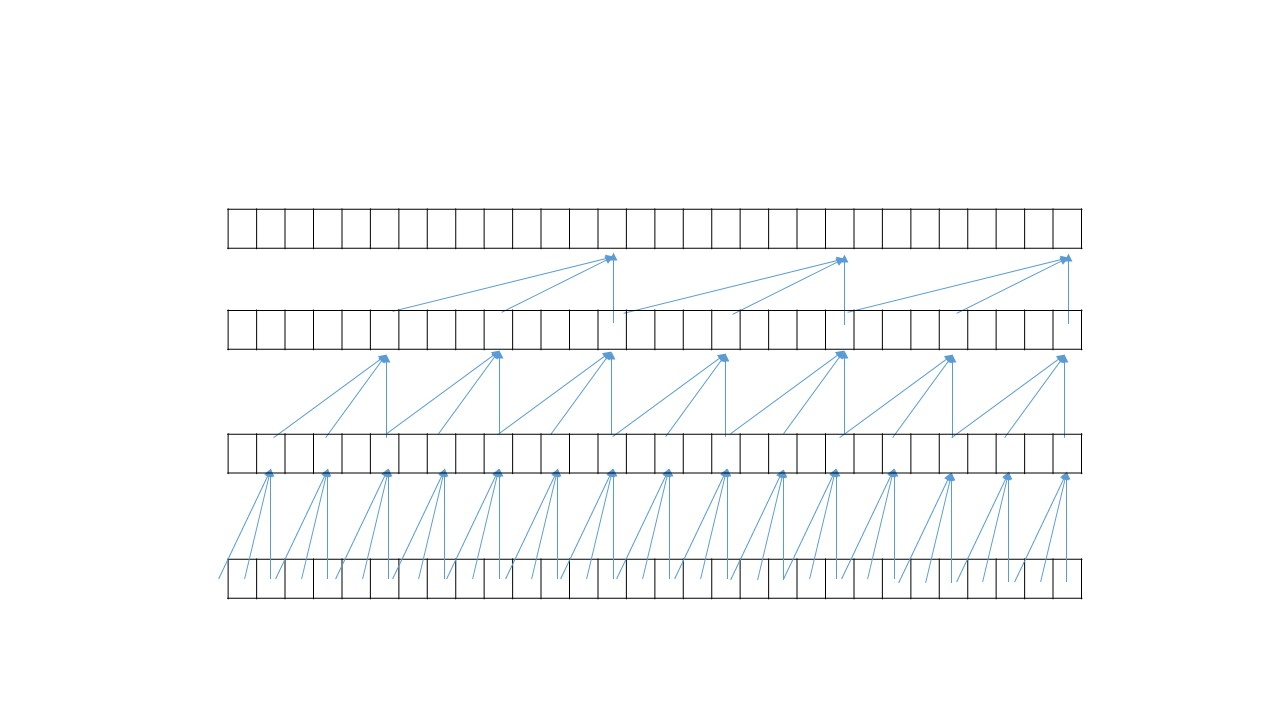
\includegraphics[width=.6\linewidth]{./fig/TCN_model} 

}

\caption{時序卷積網絡}\label{fig:TCNmodel}
\end{figure}

\hypertarget{ux6642ux5e8fux5377ux7a4dux7db2ux7d61ux8207ux5b63ux7bc0ux6027ux81eaux8ff4ux6b78}{%
\subsection{時序卷積網絡與季節性自迴歸}\label{ux6642ux5e8fux5377ux7a4dux7db2ux7d61ux8207ux5b63ux7bc0ux6027ux81eaux8ff4ux6b78}}

本研究發現,若將SARIMA模型去除季節性因素後,其表現與類神經網絡無太大差別,從\ref{tab:RMSE} 中,短期數的預測與LSTM模型相去不遠。因此推測若將時序卷機網絡加進季節性因素,可以提升網絡的預測能力。

因此本研究在時序卷積網絡再增加季節性參數,令k為卷積核大小、d為膨脹因子,以(k,d)表示,此外令p=12表週期大小。如圖@re(fig:STCNmodel)所示,將三個卷積層(3,1)、(2,p-1)、(2,p)由下而上的相疊,目的是期望能仿照ARIMA(2,0,0)(2,0,0)的感受域。以下將說明雙時序網絡如何包含ARIMA(2,0,0)(2,0,0)的感受域,由最下層依序往上的卷積核分別為,\(\omega^{0}=(\omega^{0}_0,\omega^{0}_1,\omega^{0}_2)\)、\(\omega^{1}=(\omega^{1}_0,\omega^{1}_1)\)、\(\omega^{2}=(\omega^{2}_0,\omega^{2}_1)\),其中上標\((i)\)表示第幾層,0為第一層,2為最上層。假設有一時間序列\(z=\{z_t\}^{T-1}_{t=0}\),經過第0層卷積層的產出可表示為,

\[(\omega^{(0)}*z)(t)=\omega^{(0)}_0z_t+\omega^{(0)}_1z_{t-1}+\omega^{(0)}_2z_{t-2}\]

再將第0層產出套入第一層卷積後的結果可表示為,

\[\omega^{(1)}[\omega^{(0)}_0z_t+\omega^{(0)}_1z_{t-1}+\omega^{(0)}_2z_{t-2}]+\omega^{(1)}[\omega^{(0)}_0z_{t-(p-1)}+\omega^{(0)}_1z_{t-p}+\omega^{(0)}_2z_{t-(p+1)}]\]

\begin{align*}
(\omega^{(1)}*\omega^{(0)}*z)(t)&=\omega^{(1)}(\omega^{(0)}*z)(t)+\omega^{(1)}(\omega^{(0)}*z)(t-(p-1)) \\
      &= \omega^{(1)_0}[\omega^{(0)}_0z_t+\omega^{(0)}_1z_{t-1}+\omega^{(0)}_2z_{t-2}] \\
      &+\omega^{(1)}_1[\omega^{(0)}_0z_{t-(p-1)}+\omega^{(0)}_1z_{t-p}+\omega^{(0)}_2z_{t-(p+1)}]
\end{align*}

再將上式套入第2個卷積層

\begin{align*}
(\omega^{(2)}*\omega^{(1)}*\omega^{(0)}*z)(t) &=\omega^{(2)}(\omega^{(1)}*\omega^{(0)}*z)(t)+\omega^{(2)}(\omega^{(1)}*\omega^{(0)}*z)(t-p)\\
&= \omega^{(2)}_0\omega^{(1)}_0[\omega^{(0)}_0z_t+\omega^{(0)}_1z_{t-1}+\omega^{(0)}_2z_{t-2}]\\
      &+\omega^{(2)}_0\omega^{(1)}_1[\omega^{(0)}_0z_{t-(p-1)}+\omega^{(0)}_1z_{t-p}+\omega^{(0)}_2z_{t-(p+1)}]\\
      &+\omega^{(2)}_1\omega^{(1)}_0[\omega^{(0)}_0z_{t-p}+\omega^{(0)}_1z_{t-(p+1)}+\omega^{(0)}_2z_{t-(p+2)}]\\
      &+\omega^{(2)}_1\omega^{(1)}_1[\omega^{(0)}_0z_{t-(2p-1)}+\omega^{(0)}_1z_{t-2p}+\omega^{(0)}_2z_{t-(2p+1)}]
\end{align*}

經整理後可寫為,

\begin{align*}
(\omega^{(2)}*\omega^{(1)}*\omega^{(0)}*z)(t) &=\omega^{(2)}_0\omega^{(1)}_0[\omega^{(0)}_0z_t+\omega^{(0)}_1z_{t-1}+\omega^{(0)}_2z_{t-2}]\\
&+\omega^{(2)}_0\omega^{(1)}_0\omega^{(0)}_0z_{t-(p-1)}+(\omega^{(2)}_0\omega^{(1)}_1\omega^{(0)}_1+\omega^{(2)}_1\omega^{(1)}_0\omega^{(0)}_0)z_{t-p}\\
&+(\omega^{(2)}_0\omega^{(1)}_1\omega^{(0)}_2+\omega^{(2)}_1\omega^{(1)}_0\omega^{(0)}_1)z_{t-(p+1)}+\omega^{(2)}_1\omega^{(1)}_0\omega^{(0)}_2)z_{t-(p+2)}\\
&+\omega^{(2)}_1\omega^{(1)}_1[\omega^{(0)}_0z_{t-(2p-1)}+\omega^{(0)}_1z_{t-2p}+\omega^{(0)}_2z_{t-(2p+1)}]
\end{align*}

對比於\(ARIMA(2,0,0)(2,0,0)_p\)的感受域,

\[(1-\phi_1B-\phi_2B^2)(1-\Phi_1B^p-\Phi_2B^{2p})z_{t+1}=\epsilon_{t+1}\]
把落後項因子展開,

\begin{align*}
(1-\phi_1B-\phi_2B^2)(1-\Phi_1B^p-\Phi_2B^{2p}) &= 1-\phi_1B-\phi_2B^2-\Phi_2B^{2p}+\phi_1\Phi_1B^{p+1}+\phi_1\Phi_2B^{2p+1}\\
&+\phi_2\Phi_1B^{p+2}+\phi_2\Phi_2B^{2p+2}
\end{align*}

式子(26)可改寫為

\[(1-\psi(B))z_{t+1} = \epsilon_{t+1}\]
可再改寫為

\[z_{t+1} = \psi(B)z_t+epsilon_{t+1}\]

其中

\[\psi(B)=\phi_1B+\phi_2B^2+\Phi_2B^{2p}-\phi_1\Phi_1B^{p+1}-\phi_1\Phi_2B^{2p+1}-\phi_2\Phi_1B^{p+2}-\phi_2\Phi_2B^{2p+2}\]

\begin{figure}

{\centering 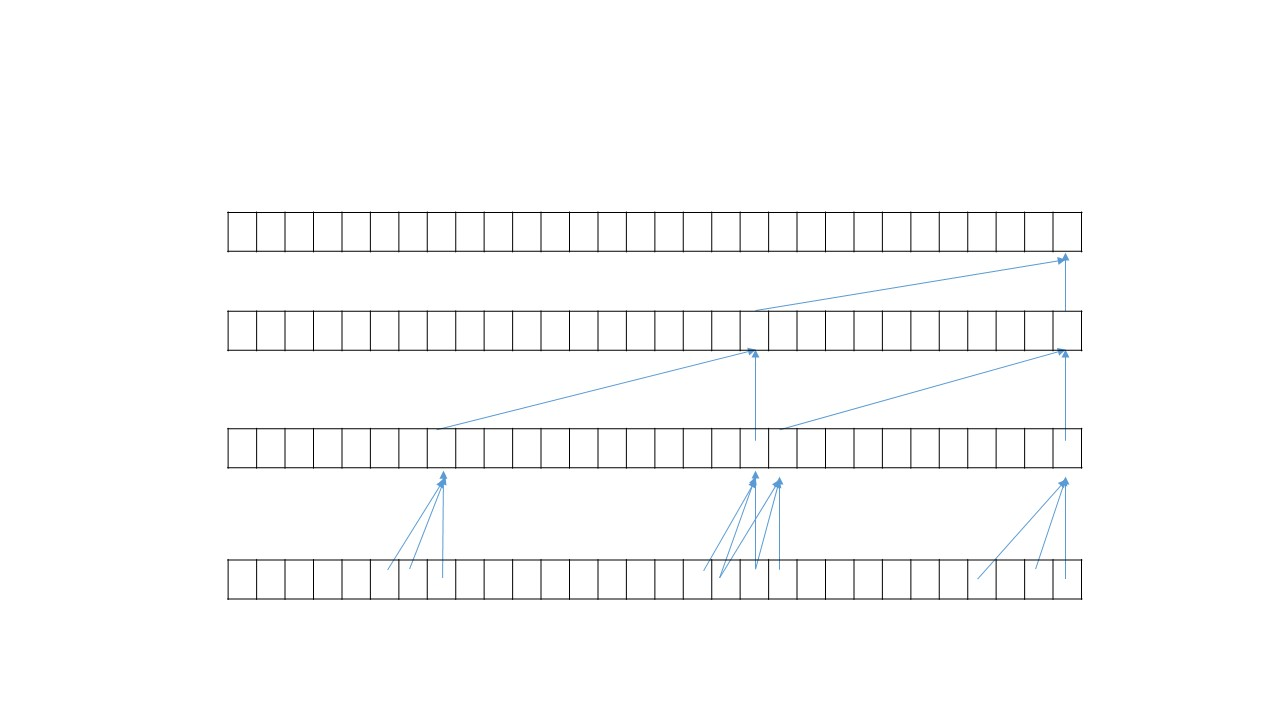
\includegraphics[width=.6\linewidth]{./fig/STCN_model} 

}

\caption{季節時序卷積網絡}\label{fig:STCNmodel}
\end{figure}

將時序卷積網絡與季節時序卷積網絡加以組合,稱為雙時序卷積網絡,比較雙時序卷積網絡(25)與\(ARIMA(2,0,0)(2,0,0)_p\)(28),可知雙時序卷積網絡多出\(z_{t-2},z_{t-(p+2)}\)兩項,由此可知雙時序卷積網絡涵蓋\(ARIMA(2,0,0)(2,0,0)_p\)的感受域。

而雙時序卷積網絡是以迭代的方式來做失業率的預測,意思是要預測h期後的失業率十,先由雙時序卷積網絡預測出一期後再迭代出2期、3期直至h期。以數學式表實則為,\((z_0,z_1,...,z_T)\)為輸入雙時序卷積網絡的時間序列,得到\(\hat{z}_{T+1|T}\) 1期後的預測,接這再將\((z_0,z_1,...,z_T,\hat{z}_{T+1|T})\)作為輸入值得到2期後預測,以此類推至h期。

\hypertarget{ux6642ux5e8fux5377ux7a4dux7db2ux7d61ux7684ux53c3ux6578ux8a2dux5b9a}{%
\subsection{時序卷積網絡的參數設定}\label{ux6642ux5e8fux5377ux7a4dux7db2ux7d61ux7684ux53c3ux6578ux8a2dux5b9a}}

此外,為了增加多層堆疊的穩定度, Bai et al. (\protect\hyperlink{ref-baiEmpiricalEvaluationGeneric2018}{2018}) 使用照 He, Zhang, Ren, \& Sun (\protect\hyperlink{ref-heDeepResidualLearning2015}{2015}) 提出的殘差區塊(residual block)的方式,建立殘差連接(residual connections)。\(o\)為網絡輸出的真實值,網絡是在學席降低\(\hat{o}\)和\(o\)間的損失值,殘差連接是將當期輸入值\(x_t\)與當期預測值\(\hat{z_t}\)做連結為一個殘差區塊,讓時序卷積網絡學習到對\(x_t\)相關資訊轉換(identity mapping)的微調,亦即\(F(x_t)\),而資料對\(\hat{z_t}\)的轉換(entire transformation)。寫成數學式如下,

\[o = Activation(x_t+F(x_t))\]

在殘差區塊中,加入整流線性單位函數(rectified linear unit, ReLU)(Nair \& Hinton, \protect\hyperlink{ref-nairRectifiedLinearUnits2010}{2010}) 在有膨脹因子的因果卷積層上,和運用權重正規化(weight normalization) (Salimans \& Kingma, \protect\hyperlink{ref-salimansWeightNormalizationSimple2016}{2016}) 在卷積網絡上。

此外,在全連接層中需要調整卷積核的個數,意味著進入全連接層前一次讀取幾層的輸入值,像是讀彩色圖片時一般會選擇卷積核個數為3,因應紅綠藍三種色彩疊層;或經過全連接層後,會產生幾個特徵值(features)。雙時序卷積網絡中,也是藉由調整卷積核的個數得到不同的特徵值,讓網絡學習進而降低損失值。

因雙時序卷積網絡是將時序卷積網絡與季節性時序卷積網絡進行組合,在參數調整上僅能調整卷積核個數,經實驗後發現卷積核個數為80時損失值最小,以此做為雙時序卷積網絡的模型參數。

\hypertarget{ux9810ux6e2cux7d50ux679cux6bd4ux8f03}{%
\chapter{預測結果比較}\label{ux9810ux6e2cux7d50ux679cux6bd4ux8f03}}

回顧資料分群方式,分做訓練、驗證及測試集,\ref{fig:TCNpred} 與\ref{fig:LSTMpred} 中以虛線將不同群分開,1978年1月至2008年3月作為訓練集,占總資料的70\%;資料2008年4月至2013年9月作為驗證集,共78筆,占總資料的15\%;資料2013年10月至2019年12月作為測試集,共75筆,占總資料的15\%。類神經網絡個別訓練1000回(epochs)。

雙時序卷積網絡是以迭代方式進行預測,將3、6、9、12個月後的失業率預測呈現,如下圖\ref{fig:TCNpred}

\begin{figure}

{\centering \subfloat[時序卷積網絡3個月後預測\label{fig:TCNpred-1}]{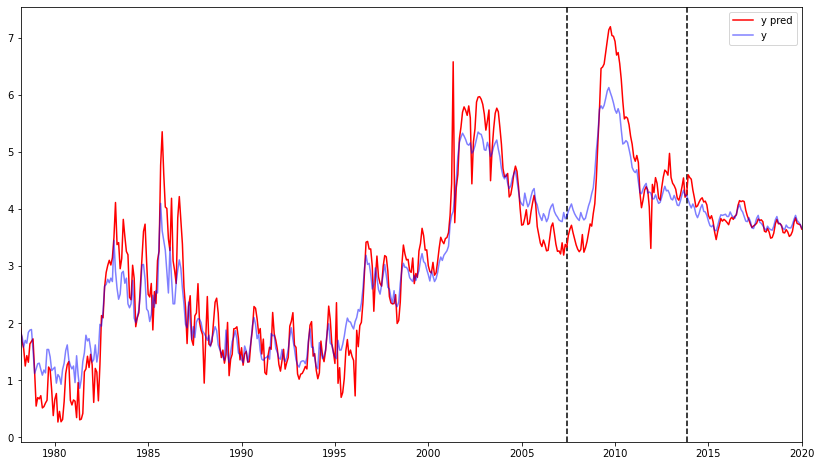
\includegraphics[width=.5\linewidth]{./fig/TCN/0112/TCN_pre3} }\subfloat[時序卷積網絡6個月後預測\label{fig:TCNpred-2}]{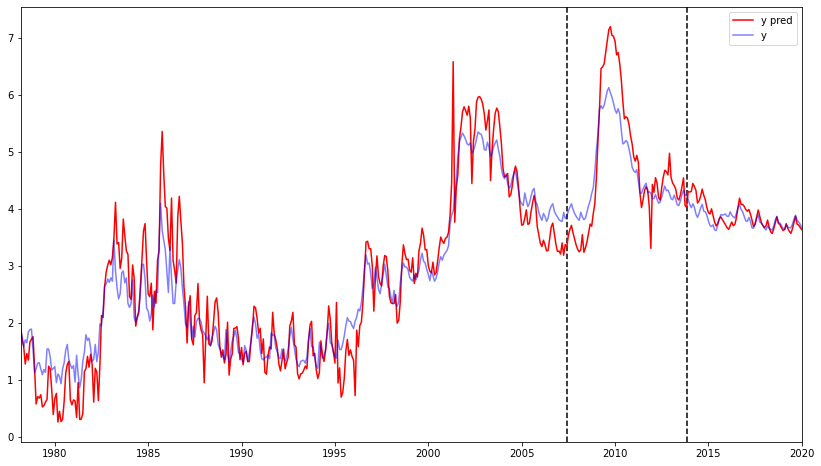
\includegraphics[width=.5\linewidth]{./fig/TCN/0112/TCN_pre6} }\newline\subfloat[時序卷積網絡9個月後預測\label{fig:TCNpred-3}]{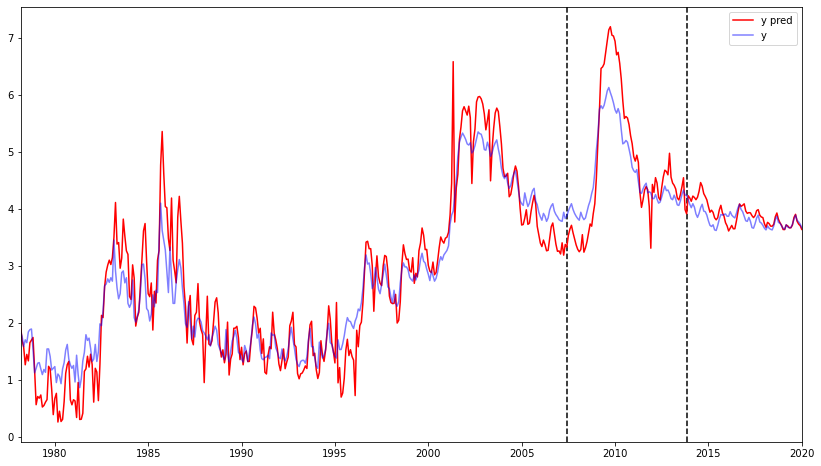
\includegraphics[width=.5\linewidth]{./fig/TCN/0112/TCN_pre9} }\subfloat[時序卷積網絡12個月後預測\label{fig:TCNpred-4}]{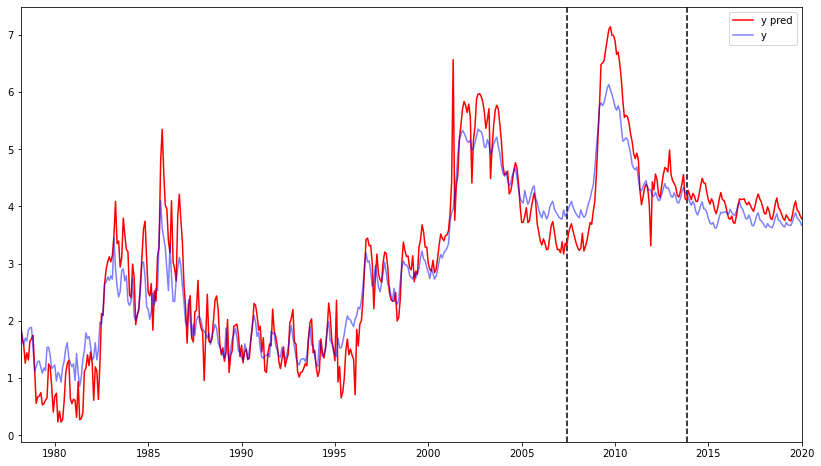
\includegraphics[width=.5\linewidth]{./fig/TCN/0112/TCN_pre12} }

}

\caption{時序卷積網絡預測}\label{fig:TCNpred}
\end{figure}

長短期記憶網絡是以直接預測數個月後的失業率,將3、6、9、12個月後的失業率預測呈現,如下圖\ref{fig:LSTMpred}

\begin{figure}

{\centering \subfloat[長短期記憶網絡3個月後預測\label{fig:LSTMpred-1}]{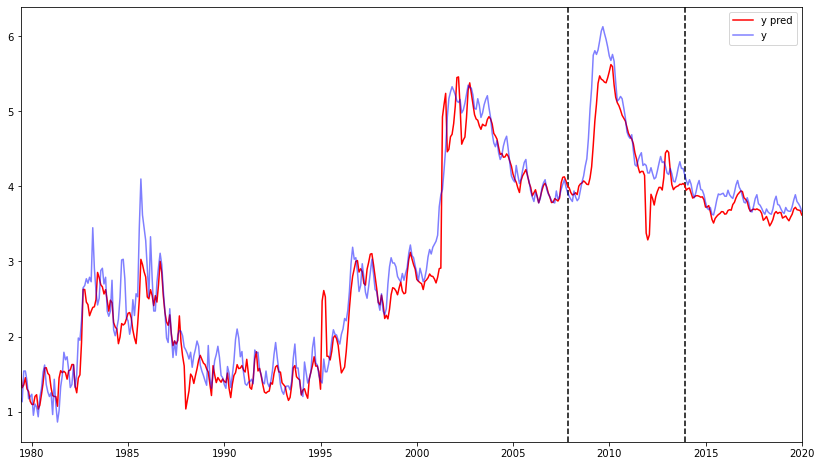
\includegraphics[width=.5\linewidth]{./fig/LSTM/0111/LSTMpre3} }\subfloat[長短期記憶網絡6個月後預測\label{fig:LSTMpred-2}]{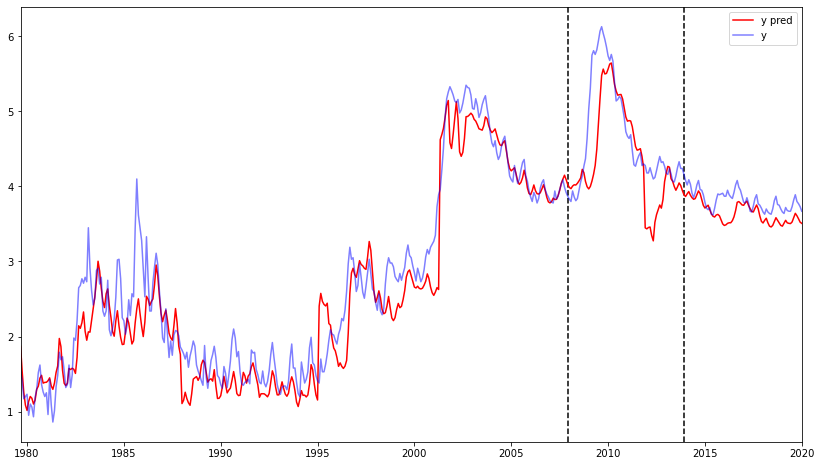
\includegraphics[width=.5\linewidth]{./fig/LSTM/0111/LSTMpre6} }\newline\subfloat[長短期記憶網絡9個月後預測\label{fig:LSTMpred-3}]{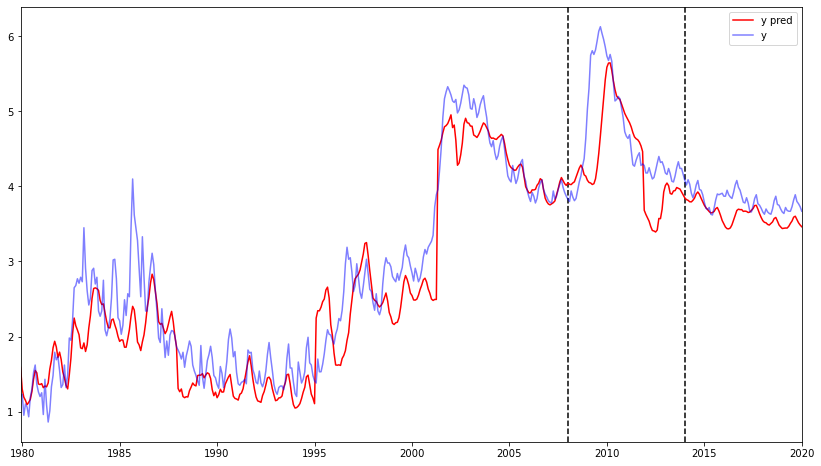
\includegraphics[width=.5\linewidth]{./fig/LSTM/0111/LSTMpre9} }\subfloat[長短期記憶網絡12個月後預測\label{fig:LSTMpred-4}]{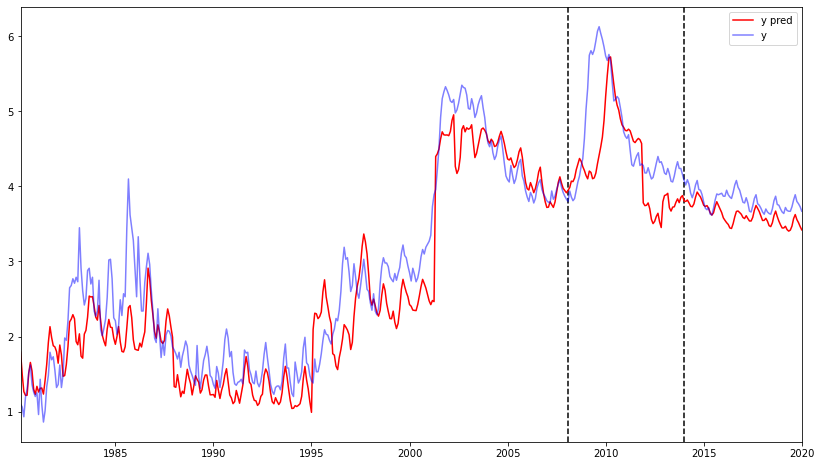
\includegraphics[width=.5\linewidth]{./fig/LSTM/0111/LSTMpre12} }

}

\caption{非同步隨機梯度下降的權重捨棄的長短期記憶網絡預測}\label{fig:LSTMpred}
\end{figure}

具結構斷裂的季節性差分整合移動平均自迴歸模型的資料分群,將訓練與測試合併為訓練集,僅有訓練集與測試集之分,\ref{fig:SARIMApred}中以虛線將不同群分開。1978年1月 \textasciitilde{} 2013年9月作為訓練集,占總資料的85\%;資料2013年10月 \textasciitilde{} 2019年12月作為測試集,共75筆,占總資料的15\%。

結構斷裂的季節性差分整合移動平均自迴歸模型是以迭代方式進行預測,將3、6、9、12個月後的失業率預測呈現,如下圖\ref{fig:SARIMApred}

\begin{figure}

{\centering \subfloat[SARIMAX3個月後\label{fig:SARIMApred-1}]{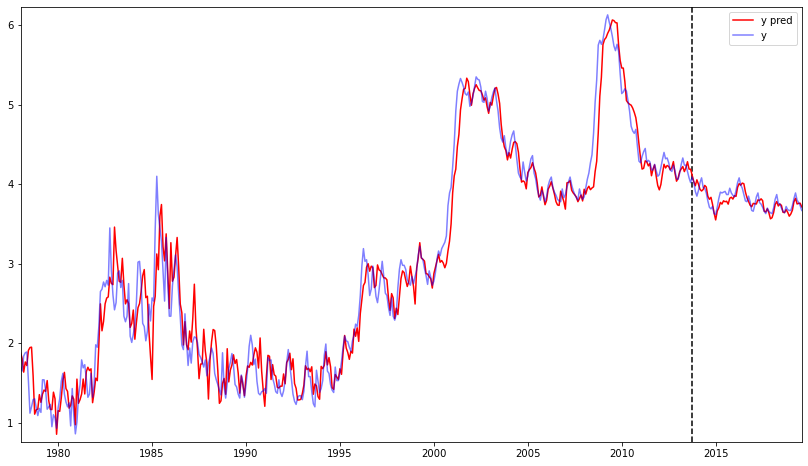
\includegraphics[width=.5\linewidth]{./fig/ARIMA/arima_f3} }\subfloat[SARIMAX6個月後預測\label{fig:SARIMApred-2}]{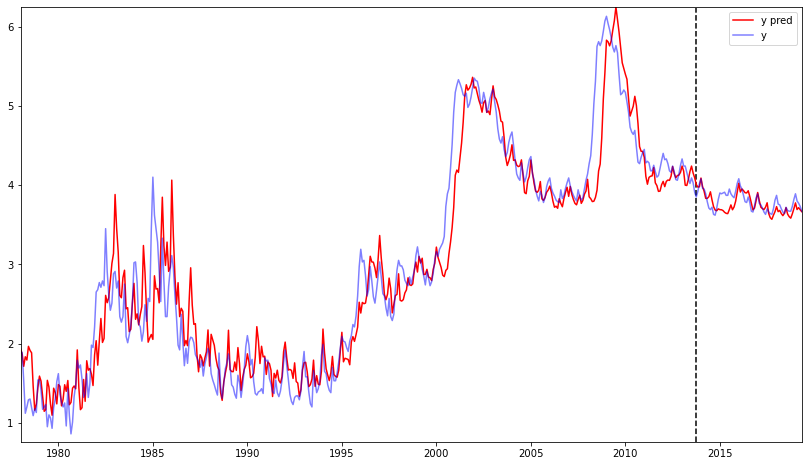
\includegraphics[width=.5\linewidth]{./fig/ARIMA/arima_f6} }\newline\subfloat[SARIMAX9個月後預測\label{fig:SARIMApred-3}]{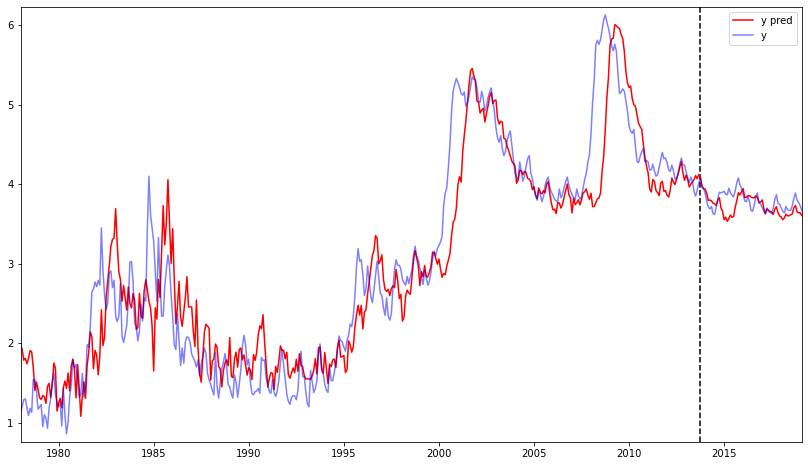
\includegraphics[width=.5\linewidth]{./fig/ARIMA/arima_f9} }\subfloat[SARIMAX12個月後預測\label{fig:SARIMApred-4}]{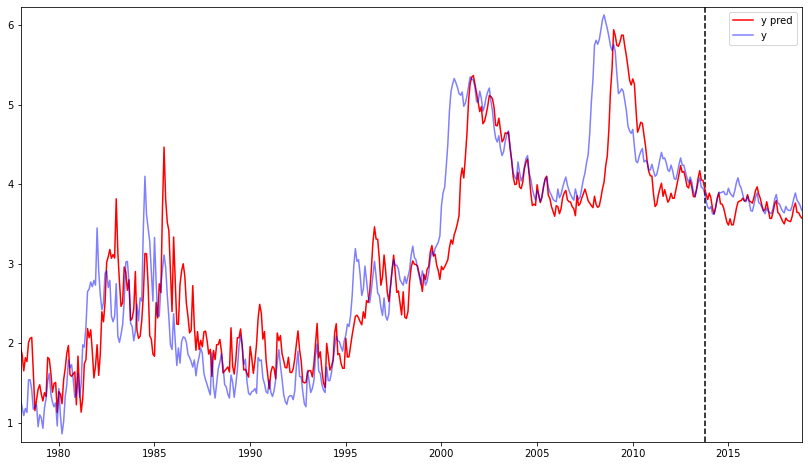
\includegraphics[width=.5\linewidth]{./fig/ARIMA/arima_f12} }

}

\caption{具結構斷裂的季節性差分整合移動平均自迴歸模型預測}\label{fig:SARIMApred}
\end{figure}

\hypertarget{ux6bd4ux8f03ux5177ux7d50ux69cbux65b7ux88c2ux7684ux5b63ux7bc0ux6027ux5deeux5206ux6574ux5408ux79fbux52d5ux5e73ux5747ux81eaux8ff4ux6b78ux6a21ux578bux985eux795eux7d93ux7db2ux7d61ux7684ux6a23ux672cux5916ux9810ux6e2cux7684ux5747ux65b9ux6839ux8aa4ux5dee}{%
\section{比較具結構斷裂的季節性差分整合移動平均自迴歸模型、類神經網絡的樣本外預測的均方根誤差}\label{ux6bd4ux8f03ux5177ux7d50ux69cbux65b7ux88c2ux7684ux5b63ux7bc0ux6027ux5deeux5206ux6574ux5408ux79fbux52d5ux5e73ux5747ux81eaux8ff4ux6b78ux6a21ux578bux985eux795eux7d93ux7db2ux7d61ux7684ux6a23ux672cux5916ux9810ux6e2cux7684ux5747ux65b9ux6839ux8aa4ux5dee}}

透過樣本外預測的均方根誤差,藉由模型預測值與實際值間的落差,來衡量模型的好壞。本研究是以測試集的失業率,也就是2013年10月至2019年12月作為樣本外預測的資料,以數學式表示,均方根誤差(root mean square error, RMSE)

\[\sqrt{\frac{\sum_{t=1}^n(\hat{y_t}-y_t)}{n}}\]

\begin{table}

\caption{\label{tab:RMSE}樣本外預測的均方根誤差}
\centering
\begin{tabular}[t]{r|r|r|r|r|r}
\hline
幾個月後預測 & SARIMAX & STCN & AWDLSTM & ARIMAX & TCN\\
\hline
1 & 0.04 & 0.04 & 0.07 & 0.06 & 0.05\\
\hline
2 & 0.06 & 0.06 & 0.11 & 0.10 & 0.07\\
\hline
3 & 0.08 & 0.08 & 0.13 & 0.13 & 0.08\\
\hline
4 & 0.09 & 0.09 & 0.16 & 0.14 & 0.09\\
\hline
5 & 0.10 & 0.10 & 0.19 & 0.15 & 0.10\\
\hline
6 & 0.11 & 0.11 & 0.20 & 0.15 & 0.11\\
\hline
7 & 0.12 & 0.12 & 0.21 & 0.16 & 0.11\\
\hline
8 & 0.13 & 0.12 & 0.22 & 0.16 & 0.12\\
\hline
9 & 0.14 & 0.13 & 0.22 & 0.16 & 0.11\\
\hline
10 & 0.15 & 0.16 & 0.22 & 0.16 & 0.12\\
\hline
11 & 0.16 & 0.13 & 0.22 & 0.16 & 0.13\\
\hline
12 & 0.16 & 0.17 & 0.23 & 0.15 & 0.13\\
\hline
\end{tabular}
\end{table}

從表\ref{tab:RMSE},比較均方根誤差,雙時序卷積網絡(STCN),除了在一個月後預測比SARIMA模型差,其餘幾個月後的預測皆為最佳。而長短期(AWDLSTM)模型的表現遜色於雙時序卷積網絡、SARIMA模型、ARIMAX。時序卷積網絡(TCN)預測能力,稍落後SARIMA模型,但考量季節性變化後的雙時序卷積網絡,則優於SARIMA模型。
從SARIMA與ARIMAX間、雙時序卷積網絡與時序卷積網絡間,可以看到考慮失業率的季節性後,確實可以讓預測能力有所提升。

\hypertarget{ux985eux795eux7d93ux7db2ux7d61ux7684ux8a13ux7df4ux72c0ux6cc1}{%
\section{類神經網絡的訓練狀況}\label{ux985eux795eux7d93ux7db2ux7d61ux7684ux8a13ux7df4ux72c0ux6cc1}}

類神經網絡可以透過驗證集損失函數(loss function) 的變化,來了解模型是否有過度擬合的問題,當驗證集的損失函數沒有隨著訊連次數提升而下降,反而驗證集的損失函數值隨著時間遞增,就存在過度擬合的問題。而驗證集的損失函數值與訓練集的損失函數值水準值的高低,代表不同的輸入值所產生的損失函數的不同,不意味著存有過度擬合的問題。
對於圖\ref{fig:LSTMloss}非同步隨機梯度下降的權重捨棄的長短期記憶網絡,不論3、6、9、12個月後的預測的模型,其驗證集的損失函數值都有隨著訓練次數增加而遞減未反映出過度訓練。對於圖\ref{fig:TCNloss}TCN模型不論3、6、9、12個月後的預測的模型,亦未有過度訓練的問題。

\begin{figure}

{\centering \subfloat[長短期記憶網絡3個月後預測訓練誤差變化\label{fig:LSTMloss-1}]{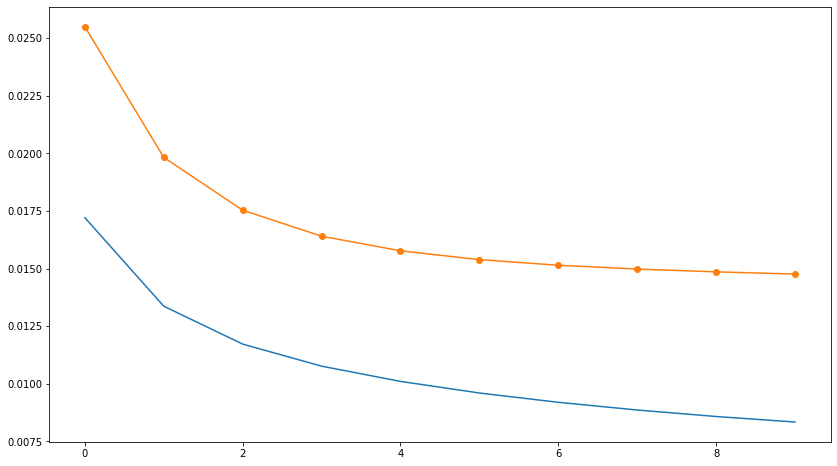
\includegraphics[width=.5\linewidth]{./fig/LSTM/0111/LSTMloss3} }\subfloat[長短期記憶網絡6個月後預測訓練誤差變化\label{fig:LSTMloss-2}]{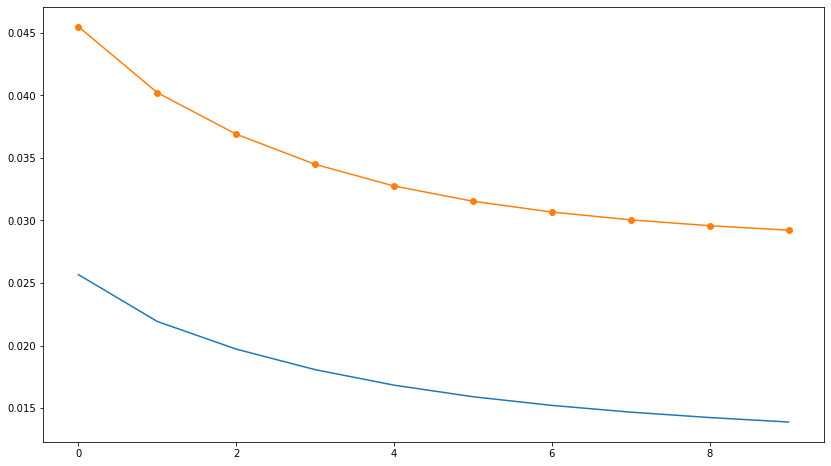
\includegraphics[width=.5\linewidth]{./fig/LSTM/0111/LSTMloss6} }\newline\subfloat[長短期記憶網絡9個月後預測訓練誤差變化\label{fig:LSTMloss-3}]{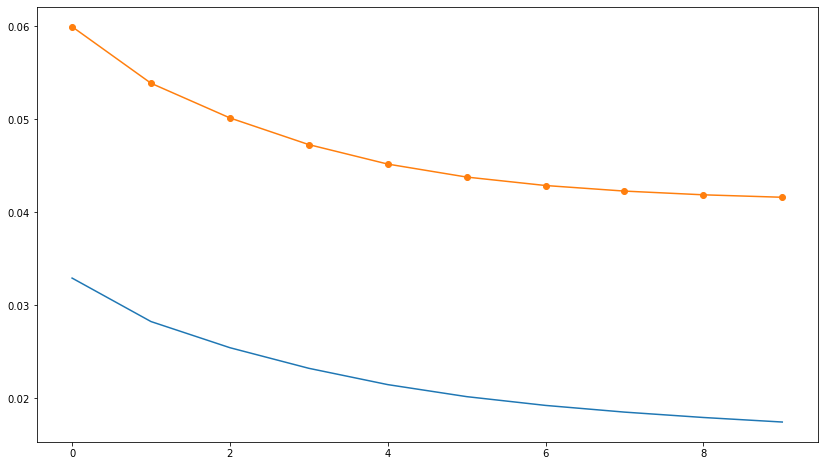
\includegraphics[width=.5\linewidth]{./fig/LSTM/0111/LSTMloss9} }\subfloat[長短期記憶網絡12個月後預測訓練誤差變化\label{fig:LSTMloss-4}]{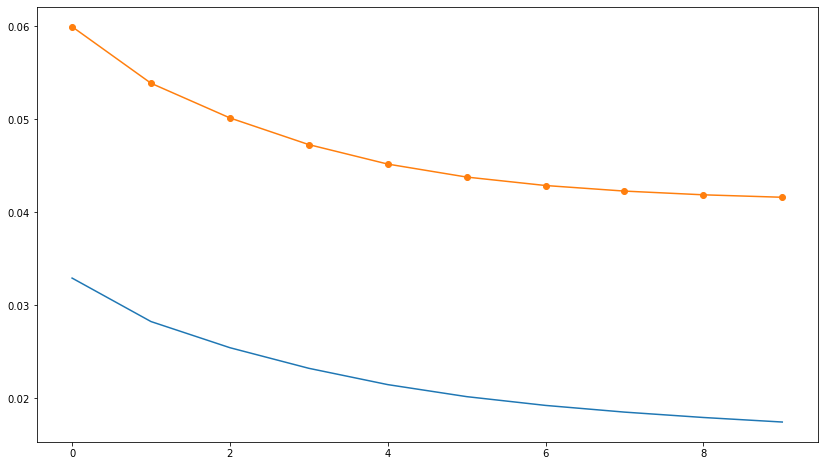
\includegraphics[width=.5\linewidth]{./fig/LSTM/0111/LSTMloss9} }

}

\caption{非同步隨機梯度下降的權重捨棄的長短期記憶網絡的訓練誤差變化}\label{fig:LSTMloss}
\end{figure}

\begin{figure}

{\centering \subfloat[時序卷積網絡3個月後預測訓練誤差變化\label{fig:TCNloss-1}]{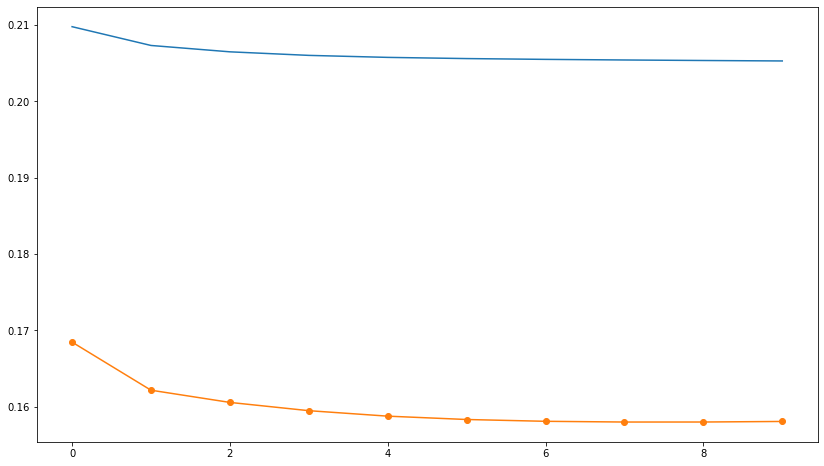
\includegraphics[width=.5\linewidth]{./fig/TCN/0112/TCN_loss3} }\subfloat[時序卷積網絡6個月後預測訓練誤差變化\label{fig:TCNloss-2}]{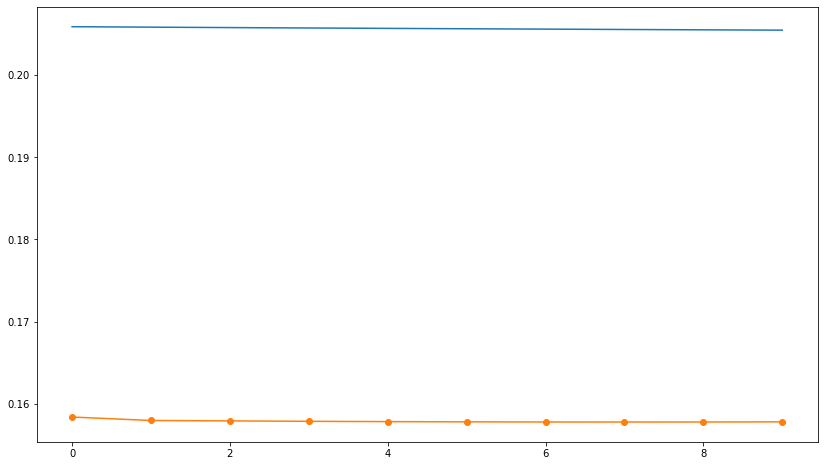
\includegraphics[width=.5\linewidth]{./fig/TCN/0112/TCN_loss6} }\newline\subfloat[時序卷積網絡9個月後預測訓練誤差變化\label{fig:TCNloss-3}]{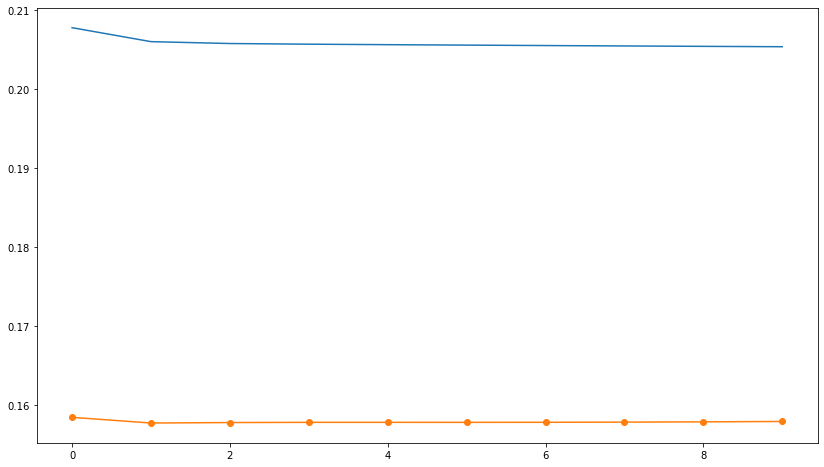
\includegraphics[width=.5\linewidth]{./fig/TCN/0112/TCN_loss9} }\subfloat[時序卷積網絡12個月預測後訓練誤差變化\label{fig:TCNloss-4}]{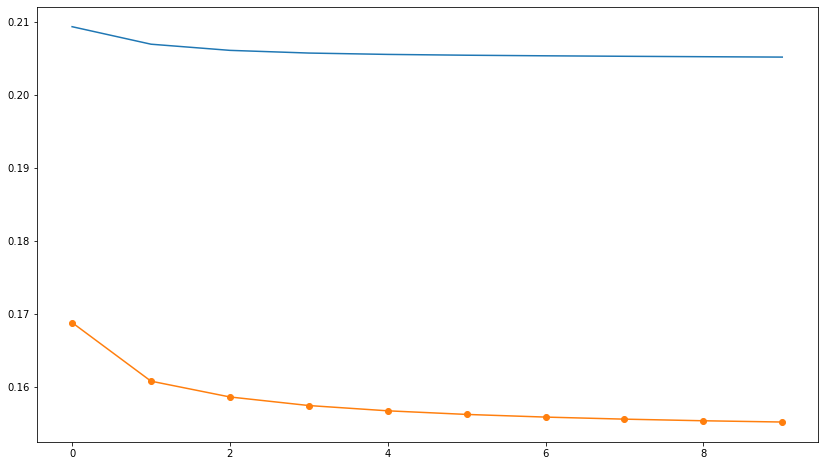
\includegraphics[width=.5\linewidth]{./fig/TCN/0112/TCN_loss12} }

}

\caption{時序卷積網絡的訓練誤差變化}\label{fig:TCNloss}
\end{figure}

\hypertarget{ux7d50ux8ad6}{%
\chapter{結論}\label{ux7d50ux8ad6}}

殺雞焉用牛刀,或許是本研究對單變數失業率預測的註解,類神經網絡不見得在所有時候,都會有較好的表現。但預測是種參數估計,從三個模型中可以了解到,不同模型對同樣一筆失業率資料有不同參數選擇與估計的方法,因而對資料的生成方式有不同的解,影響到後續預測能力的好壞。從中可以看出長短期記憶模型與時序卷積網絡,並未對失業率的季節性做較多的著墨,但SARIMAX模型因為有捕捉到季節性的因素,而在預測上表現良好,若拿掉季節性回到ARIMA模型時,其一期後的預測能力則劣於長短期記憶模型與時序卷積網絡。

\hypertarget{ux5982ux4f55ux6539ux9032ux985eux795eux7d93ux7db2ux7d61}{%
\section{如何改進類神經網絡}\label{ux5982ux4f55ux6539ux9032ux985eux795eux7d93ux7db2ux7d61}}

後續研究在神經網絡的改進上,可著重在增加資料量或多元性、學習統計模型的特徵擷取、增加訓練次數來著手。因類神經網絡適合運用大量資料來進行模型的預估,本研究採用的失業率月資料僅有504筆,同時僅有一個失業率變數作為輸入值,若要利用類神經網絡進行經濟預測,可能需要更多元的資料輸入值,或是較多筆的資料,但有鑑於經濟資料許多為月資料甚至於季資料,在資料量上較難實現。儘管失業率的迴歸殘差\(z_t\)在非線性檢定上接近拒絕線性假設,但使用類神經網絡的表現並未明顯優於SARIMAX模型。可能是類神經網絡在做資料特徵擷取時忽略掉像是季節性因素等重要的參數,而使類神經網絡在預測上表現不特別出色,在進行類神經網絡的訓練時,應可參考統計模型,增加神經網絡對資料特徵上的認識。最後則是增加訓練次數,但同時也要留意是否有過度擬合的現象,可以藉由訓練集與驗證集的損失函數值的變化做判斷。

\hypertarget{appendix-ux9644ux9304}{%
\appendix \addcontentsline{toc}{chapter}{\appendixname}}


\hypertarget{latex-cite-pkg}{%
\chapter{LaTeX 文獻引用}\label{latex-cite-pkg}}

R Markdown 的 PDF 輸出是透過 Pandoc 的 LaTeX 模板,因此理論上 LaTeX 可以做到的事,也可以透過 R Markdown 達成。目前的問題是

\begin{quote}
LaTeX 本身並未有支援繁體中文格式的文獻引用套件
\end{quote}

經過一段時間的搜尋,發現 biblatex 套件似乎可以定義不同的引用格式\footnote{\url{https://tex.stackexchange.com/questions/417762/different-styles-between-citations-and-bibliography}~\\
  \url{https://tex.stackexchange.com/questions/377308/different-citation-styles-for-the-same-bibliography}},因此,或許可以透過定義新的標點符號,例如將原本引用格式中的\texttt{,}定義成\texttt{,}、\texttt{.}定義成\texttt{。},再透過 \texttt{.bib} 檔中的 \texttt{langid} field 辨識要使用何種引用格式。然而,由於作者本人對 LaTeX 並不熟悉,因此需要這方面高手的協助。

\renewcommand{\href}{\oldhref}

\hypertarget{references}{%
\chapter*{參考資料}\label{references}}
\addcontentsline{toc}{chapter}{參考資料}

\hypertarget{refs}{}
\leavevmode\hypertarget{ref-baiComputationAnalysisMultiple2003}{}%
Bai, J., \& Perron, P. (2003). Computation and analysis of multiple structural change models. \emph{Journal of Applied Econometrics}, \emph{18}(1), 1--22. Retrieved from \url{https://onlinelibrary.wiley.com/doi/abs/10.1002/jae.659}

\leavevmode\hypertarget{ref-baiEmpiricalEvaluationGeneric2018}{}%
Bai, S., Kolter, J. Z., \& Koltun, V. (2018). An empirical evaluation of generic convolutional and recurrent networks for sequence modeling. \emph{arXiv Preprint arXiv:1803.01271}.

\leavevmode\hypertarget{ref-bootDoesModelingStructural2020}{}%
Boot, T., \& Pick, A. (2020). Does modeling a structural break improve forecast accuracy? \emph{Journal of Econometrics}, \emph{215}(1), 35--59.

\leavevmode\hypertarget{ref-coulombeHowMachineLearning2020}{}%
Coulombe, P. G., Leroux, M., Stevanovic, D., \& Surprenant, S. (2020). How is Machine Learning Useful for Macroeconomic Forecasting?

\leavevmode\hypertarget{ref-dauphinLanguageModelingGated2017}{}%
Dauphin, Y. N., Fan, A., Auli, M., \& Grangier, D. (2017). Language Modeling with Gated Convolutional Networks. \emph{arXiv:1612.08083 {[}Cs{]}}.

\leavevmode\hypertarget{ref-dieboldPresentFutureMacroeconomic1998}{}%
Diebold, F. X. (1998). The Past, Present, and Future of Macroeconomic Forecasting. \emph{Journal of Economic Perspectives}, \emph{12}(2), 175--192. \url{https://doi.org/10.1257/jep.12.2.175}

\leavevmode\hypertarget{ref-dritsakiForecastSarimaModels2016}{}%
Dritsaki, C. (2016). Forecast of Sarima Models: Αn Application to Unemployment Rates of Greece. \emph{American Journal of Applied Mathematics and Statistics}, \emph{4}(5), 136--148.

\leavevmode\hypertarget{ref-elliottEconomicForecasting2008}{}%
Elliott, G., \& Timmermann, A. (2008). Economic Forecasting. \emph{Journal of Economic Literature}, \emph{46}(1), 3--56.

\leavevmode\hypertarget{ref-hallMacroeconomicIndicatorForecasting2017}{}%
Hall, A. S., \& Cook, T. R. (2017). \emph{Macroeconomic Indicator Forecasting with Deep Neural Networks}. Federal Reserve Bank of Kansas City.

\leavevmode\hypertarget{ref-heDeepResidualLearning2015}{}%
He, K., Zhang, X., Ren, S., \& Sun, J. (2015). Deep Residual Learning for Image Recognition. \emph{arXiv:1512.03385 {[}Cs{]}}.

\leavevmode\hypertarget{ref-hochreiterLongShortTermMemory1997}{}%
Hochreiter, S., \& Schmidhuber, J. (1997). Long Short-Term Memory. \emph{Neural Computation}, \emph{9}(8), 1735--1780. \url{https://doi.org/10.1162/neco.1997.9.8.1735}

\leavevmode\hypertarget{ref-hyndmanAutomaticTimeSeries2008}{}%
Hyndman, R. J., \& Khandakar, Y. (2008). Automatic Time Series Forecasting: The forecast Package for R. \emph{Journal of Statistical Software}, \emph{27}(1), 1--22. \url{https://doi.org/10.18637/jss.v027.i03}

\leavevmode\hypertarget{ref-kuanArtificialNeuralNetworks1994}{}%
Kuan, C.-M., \& White, H. (1994). Artificial neural networks: An econometric perspective. \emph{Econometric Reviews}, \emph{13}(1), 1--91. \url{https://doi.org/10.1080/07474939408800273}

\leavevmode\hypertarget{ref-layardUnemploymentMacroeconomicPerformance1991}{}%
Layard, R., Nickell, S., \& Jackman, R. (1991). \emph{Unemployment: Macroeconomic Performance and the Labour Market}. Oxford University Press.

\leavevmode\hypertarget{ref-leeTestingNeglectedNonlinearity1993}{}%
Lee, T. H., White, H., \& Granger, C. (1993). Testing for neglected nonlinearity in time series models: A comparison of neural network methods and alternative tests. \emph{Journal of Econometrics}, \emph{56}(3), 269--290.

\leavevmode\hypertarget{ref-lucasEconometricPolicyEvaluation1976}{}%
Lucas, R. E. (1976). Econometric policy evaluation: A critique. \emph{Carnegie-Rochester Conference Series on Public Policy}, \emph{1}, 19--46. \url{https://doi.org/10.1016/S0167-2231(76)80003-6}

\leavevmode\hypertarget{ref-merityRegularizingOptimizingLSTM2017}{}%
Merity, S., Keskar, N. S., \& Socher, R. (2017). Regularizing and Optimizing LSTM Language Models. \emph{arXiv:1708.02182 {[}Cs{]}}. Retrieved from \url{http://arxiv.org/abs/1708.02182}

\leavevmode\hypertarget{ref-montgomeryForecastingUnemploymentRate1998}{}%
Montgomery, A. L., Zarnowitz, V., Tsay, R. S., \& Tiao, G. C. (1998). Forecasting the U.S. Unemployment Rate. \emph{Journal of the American Statistical Association}, \emph{93}(442), 478--493. \url{https://doi.org/10.2307/2670094}

\leavevmode\hypertarget{ref-nairRectifiedLinearUnits2010}{}%
Nair, V., \& Hinton, G. E. (2010). Rectified Linear Units Improve Restricted Boltzmann Machines. In.

\leavevmode\hypertarget{ref-oordWaveNetGenerativeModel2016}{}%
Oord, A. van den, Dieleman, S., Zen, H., Simonyan, K., Vinyals, O., Graves, A., \ldots{} Kavukcuoglu, K. (2016). WaveNet: A Generative Model for Raw Audio. \emph{arXiv:1609.03499 {[}Cs{]}}.

\leavevmode\hypertarget{ref-salimansWeightNormalizationSimple2016}{}%
Salimans, T., \& Kingma, D. P. (2016). Weight Normalization: A Simple Reparameterization to Accelerate Training of Deep Neural Networks. \emph{arXiv:1602.07868 {[}Cs{]}}.

\leavevmode\hypertarget{ref-stockCointegrationCausalityForecasting1999}{}%
Stock, J., \& Watson, M. (1999). \emph{Cointegration, Causality and Forecasting: A Festschrift for Clive W.J. Granger}. Oxford: Oxford University Press.

\leavevmode\hypertarget{ref-swansonModelSelectionApproach1997}{}%
Swanson, N., \& White, H. (1997). A Model Selection Approach To Real-Time Macroeconomic Forecasting Using Linear Models And Artificial Neural Networks. \emph{The Review of Economics and Statistics}, \emph{79}(4), 540--550.

\leavevmode\hypertarget{ref-terasvirtaPowerNeuralNetwork1993}{}%
Teräsvirta, T., Lin, C.-F., \& Granger, C. W. J. (1993). Power of the Neural Network Linearity Test. \emph{Journal of Time Series Analysis}, \emph{14}(2), 209--220. \url{https://doi.org/https://doi.org/10.1111/j.1467-9892.1993.tb00139.x}

\leavevmode\hypertarget{ref-uscensusbureauX13ARIMASEATSSeasonalAdjustment2017}{}%
US Census Bureau, B. C. M. (2017). \emph{X-13ARIMA-SEATS Seasonal Adjustment Program}. US Census Bureau. Retrieved from \url{https://www.census.gov/srd/www/x13as/}

\leavevmode\hypertarget{ref-waibelPhonemeRecognitionUsing1989}{}%
Waibel, A., Hanazawa, T., Hinton, G., Shikano, K., \& Lang, K. J. (1989). Phoneme recognition using time-delay neural networks. \emph{IEEE Transactions on Acoustics, Speech, and Signal Processing}. Retrieved from \url{https://ieeexplore.ieee.org/document/21701}

\leavevmode\hypertarget{ref-weiTimeSeriesAnalysis2005}{}%
Wei, W. W. S. (2005). \emph{Time Series Analysis : Univariate and Multivariate Methods}. Boston.

\leavevmode\hypertarget{ref-zeileisTestingDatingStructural2003}{}%
Zeileis, A., Kleiber, C., Krämer, W., \& Hornik, K. (2003). Testing and Dating of Structural Changes in Practice. \emph{Computational Statistics \& Data Analysis}, \emph{44}, 109--123.

\leavevmode\hypertarget{ref-zhuClassNoiseVs2004}{}%
Zhu, X., \& Wu, X. (2004). Class Noise vs. Attribute Noise: A Quantitative Study. \emph{Artificial Intelligence Review}. \url{https://doi.org/10.1007/s10462-004-0751-8}

\leavevmode\hypertarget{ref-zivotFurtherEvidenceGreat1992}{}%
Zivot, E., \& Andrews, D. W. K. (1992). Further Evidence on the Great Crash, the Oil-Price Shock, and the Unit-Root Hypothesis. \emph{Journal of Business \& Economic Statistics}, \emph{10}(3), 251--270.







\end{document}
